%% Chapter 1 — Course Overview: The Big Picture of AI Services
\setcounter{chapter}{0}
\chapter{Course Overview:\\The Big Picture of AI Services}
\chaptersubtitle{Develop → Train → Serve → Operate — and the cloud underneath it all}

\begin{calloutbox}{tbbblue}{tbbbluefill}
{\normalsize\bfseries\color{tbbblue}Learning objectives}\par\vspace{3pt}
\begin{tbbitemize}
  \item Explain, from a demo night gone wrong and one month-end cloud bill, the gap between a well-trained model and an AI service that actually operates in production — and why not one of the questions that gap raises is about accuracy.
  \item Draw the full AI service stack (develop → train → serve → operate) and connect each stage to its activities, artifacts, and infrastructure needs.
  \item Compare training and inference workloads along six or more dimensions, and discuss how those differences shape infrastructure design.
  \item Use the \textbf{serving triangle} — latency, throughput, cost — to name what any given optimization pays and what it buys, and explain why an SLO is a point on that triangle chosen on purpose.
  \item Explain why an inference server's memory use is spiky rather than flat, and why sizing it by "observed idle + 10\%" is a recipe for trouble.
  \item Reinterpret the classic cloud service models (IaaS · PaaS · SaaS) from an AI-infrastructure point of view, read the GPUaaS and model-API ecosystem, and argue the "serve it yourself vs. buy an API" decision with the criteria — and the meters — that actually decide it.
\end{tbbitemize}
\end{calloutbox}

\vspace{5.0pt}

\begin{calloutbox}{tbbteal}{tbbtealfill}
{\normalsize\bfseries\color{tbbteal}Key terms}\par\vspace{3pt}
AI service stack · serving · inference · workload · latency · tail latency (p95/p99) · throughput · the serving triangle · SLO · utilization · replica · IaaS/PaaS/SaaS · GPUaaS · neocloud · serverless GPU · model API · tokens, keys, and quotas · open-weight models · build vs. buy
\end{calloutbox}

\vspace{5.0pt}

\begin{calloutbox}{tbblightgray}{tbbboxfill}
{\normalsize\bfseries\color{tbbink}Chapter outline}\par\vspace{3pt}
\textbf{1.1} From model to service: why study "serving systems"    \textbf{1.2} The full AI service stack    \textbf{1.3} Training vs. inference workloads — and the serving triangle    \textbf{1.4} Cloud service models and AI infrastructure    \textbf{1.5} The GPUaaS and model-API ecosystem    \textbf{1.6} Course roadmap and how to study — followed by a summary, exercises, and further reading.
\end{calloutbox}

\section{From Model to Service: Why Study "Serving Systems"}

Before this course teaches you a single tool, it owes you the reason the tools exist. So we open not with definitions but with two exhibits and one world-famous story. The exhibits are composites — every engineering program produces a version of them each year — but every number in them is arithmetically honest, and by the end of this section you will be able to do the arithmetic yourself. The story is entirely real.

\subsection*{Exhibit A: demo night}

A three-person course team has spent the semester building an image-captioning model. Validation accuracy: 94\%. On the team laptop, a photo goes in and a caption comes out in a third of a second. At 21:04 on demo night, they post the link to the department Discord. What follows is reconstructed from the terminal:

\begin{terminalbox}
\begin{Verbatim}[breaklines=true,breakanywhere=true,fontsize=\small,formatcom=\color{tbbtermfg},codes=\tbbcodeactive]
$ curl -w "%{time_total}s\n" -o /dev/null -s localhost:8000/caption -d @cat.jpg
0.31s                          # my laptop. instant. ship it.
# 21:04  posted the demo link to the department discord
# 21:11  "it's loading for me"  "same"  "is it down?"
$ hey -z 30s -c 100 http://demo.example.edu/caption   # 100 concurrent users
Summary:
  Requests/sec:  3.2
  Latency   p50: 15.2s    p95: 28.9s    p99: 30.0s
  Error distribution:
  [504] Gateway Timeout: 61 responses
# 21:19  the server never crashed. it queued.
# accuracy is still 94%. nobody stayed to find out.
\end{Verbatim}
\end{terminalbox}
\figcaption{Exhibit 1-A  Demo night, reconstructed. One GPU, one request at a time, one hundred users. The model did nothing wrong — and the service failed anyway.}

Do the autopsy with arithmetic, because the arithmetic is the whole story. The server handles \textbf{one request at a time}, and each takes 0.31 seconds — so its ceiling is 1 ÷ 0.31 ≈ \textbf{3.2 requests per second}, exactly the throughput \code{hey} measured. With 100 users holding connections open, a new arrival joins a queue roughly fifty deep on average: 50 × 0.31 ≈ \textbf{15.5 seconds of waiting} before its own 0.31 seconds of work — there is the p50. The unluckiest requests queue behind ninety-nine others: 99 × 0.31 ≈ 30.7 seconds — but the gateway in front gives up at 30, so they die as \textbf{504s} instead. Nothing crashed; nothing was misconfigured in the usual sense. A service with a hard ceiling of 3.2 requests per second met 100 concurrent users, and queueing theory did the rest. (This little ceiling-and-queue calculation returns formally in Week 7 — it is called Little's Law, and you will use it to size real fleets in Weeks 9 and 12.)

Notice, too, what the team knew and when. The first signal that anything was wrong was \textbf{friends complaining in chat at 21:11} — seven minutes of silent failure, because a laptop terminal showing "200 OK" lines is not monitoring. And notice the phrase the team said at 21:20, which you have already guessed: \textit{"but it works on my machine."} Hold that phrase; Chapter 4 opens with an entire dramatization of it, one layer further down.

\subsection*{Exhibit B: the bill arrives anyway}

Chastened, the team does the obvious next thing: they rent a proper GPU machine in the cloud, redeploy, and demo successfully to their advisor that Friday. Everyone graduates to other deadlines. The machine does not. At month's end, the cloud console reports:

\begin{terminalbox}
\begin{Verbatim}[breaklines=true,breakanywhere=true,fontsize=\small,formatcom=\color{tbbtermfg},codes=\tbbcodeactive]
# Billing > Bills > October (excerpt)
Amazon EC2   g5.xlarge (1x NVIDIA A10G, 24 GB)   us-east-1
   744 hrs x $1.006/hr                        $748.46
EBS storage + data transfer                    $31.20
                                     TOTAL    $779.66
# total time the demo was actually used, all month: ~90 minutes.
# utilization: 1.5 hrs / 744 hrs = 0.2%. the meter does not care.
\end{Verbatim}
\end{terminalbox}
\figcaption{Exhibit 1-B  The month-end bill for a demo that was used for ninety minutes. An always-on GPU bills 744 hours a month whether requests arrive or not.}

This exhibit's autopsy needs no queueing theory, just one multiplication: a GPU instance is billed \textbf{by the hour, for every hour it exists} — 24 × 31 = 744 of them in October — and the meter is entirely indifferent to whether inference happened. Utilization of 0.2\% means the team paid roughly \textbf{\$8.66 per minute of actual use}. The two exhibits are mirror images: Exhibit A is what happens when demand exceeds the capacity you provisioned; Exhibit B is what you pay when the capacity you provisioned exceeds demand. Steering between them — continuously, automatically, as traffic breathes — is called autoscaling, it is Week 12, and it is much harder than it sounds because a GPU serving instance takes minutes, not milliseconds, to come back (the \textit{cold start} problem). For now, keep the pair of exhibits as the course's two poles: \textbf{too slow} and \textbf{too expensive}.

\begin{calloutbox}{tbbamber}{tbbamberfill}
{\normalsize\bfseries\color{tbbamberdark}The questions that arrived between 21:04 and the end of the month}\par\vspace{3pt}
\begin{tbbitemize}
  \item \textbf{Concurrency} — What happens when 100 users send requests at the same moment? Exhibit A's answer: they form a queue behind a 3.2 req/s ceiling. What would yours be?
  \item \textbf{Latency} — Inference took 0.31 s on the laptop. Why did the median user wait 15 s? Why is the \textit{worst} user's experience (p99) the number that matters?
  \item \textbf{Availability} — If the server process dies at 3 a.m., who restarts it? What do users see in the meantime?
  \item \textbf{Cost} — Exhibit B's answer to "will you keep the GPU running through the night?" was "yes, by default, at \$1.006/hr." What is yours?
  \item \textbf{Deployment} — A better model is ready. How do you swap it in without stopping the service — and roll back when it misbehaves?
  \item \textbf{Observability} — The team's monitoring system was \textit{friends complaining in chat}. What should it have been?
\end{tbbitemize}
\end{calloutbox}

\vspace{3.0pt}

What do these six questions have in common? \textbf{Not one of them is about the model's accuracy.} They are all questions about systems. Pushing a 94\%-accurate model to 96\% is a machine learning problem; answering the six questions above belongs to operating systems, networking, distributed systems, and cloud infrastructure. The latter is what this course is about.

\subsection*{The most famous serving story ever told}

If the exhibits feel student-sized, scale them up by seven orders of magnitude and you get the most consequential product launch of the decade. On \textbf{November 30, 2022}, OpenAI released ChatGPT, describing it modestly as a "research preview." Five days later it had a million users. By January it had an estimated hundred million monthly users — analysts at the time called it the fastest-growing consumer application in history (the comparison chart that circulated everywhere: about 2.5 months for Instagram to reach one million users, 3.5 \textit{years} for Netflix). And through that first winter, the most-shared screenshot was not a clever answer but an error page: \textbf{"ChatGPT is at capacity right now"}, decorated with limericks the model had written about its own overload. Exhibit A, planet-sized: demand exceeding provisioned capacity, dramatized for a hundred million people.

Here is the detail that makes the story belong to this chapter rather than to a machine learning course: \textbf{the model was not the news.} The GPT-3 family had been publicly available through an API for over two years; the underlying capability of ChatGPT's launch model was essentially that of models developers already had access to. What launched on November 30 was \textit{packaging and serving}: a chat interface, free access, and the infrastructure ambition to put a large language model in front of everyone on earth at once. The gap between "the capability exists behind an API" and "my parents use it" turned out to be worth, by later valuations, hundreds of billions of dollars — and that gap is made of precisely the six questions in the box above, asked at planetary scale. Exhibit B scaled up too: within days, OpenAI's CEO publicly admitted the compute costs were "eye-watering," and two months later the \$20-per-month Plus tier appeared. Serving cost is never a footnote; at scale it writes the business model.

\subsection*{The model is a small part of the service}

None of this was a surprise to systems engineers, because the pattern predates LLMs. Its most famous statement is the 2015 Google paper "Hidden Technical Debt in Machine Learning Systems." In its iconic figure, when you draw an entire production ML system, the "ML code" at the center is a tiny black box surrounded by much larger boxes: data collection, feature extraction, serving infrastructure, monitoring, resource management, configuration. In the paper's phrasing, ML code is "at most 5\%" of a mature system; the other 95\% is plumbing — that is, systems.

A decade later, in the era of large language models, the ratio has become more extreme, not less. Many teams no longer train models at all; they take publicly released pretrained models off the shelf. Once the model itself is "a given," what separates teams is \textbf{how fast, how reliably, and how cheaply they can turn that model into a service.} Two teams serving the same open-source model can end up worlds apart: one responds in 4 seconds and burns \$8,000 a month; the other responds in half a second at a fifth of the cost. The knowledge that creates that gap is the content of this course.

\subsection*{The stance of this course: start from principles}

There are two ways to teach serving systems. One is tool-first: learn Docker commands and Kubernetes YAML quickly and get something deployed. The other is principles-first: understand which kernel mechanisms those tools stand on before touching them. This course takes the second path. We will spend the first six weeks digging into hypervisors, Linux namespaces, cgroups, and container runtimes at the kernel level — for two reasons.

First, \textbf{tools change; principles remain.} By the time you graduate, some orchestrator more fashionable than Kubernetes may well exist. But it, too, will implement isolation with namespaces and resource limits with cgroups. If you know the principles, every new tool is just "a new wrapper around concepts I already know."

Second, \textbf{failures happen where abstractions leak.} Most days you can happily treat a container as a "lightweight VM." That changes the day your inference server keeps dying with no visible cause and a cryptic \code{exit code 137} in the logs. Only someone who knows that a container's memory limit is a kernel cgroup — and that the moment a process crosses it, the kernel's OOM killer sends SIGKILL, which is signal 9, which is 128 + 9 = 137 — can explain why the server vanished without leaving a single log line, and fix it. You will inflict exactly this death on your own process in the Week 3 lab, on purpose, and the number 137 will follow you helpfully for the rest of the course.

In short, this is not a course about \textit{building} AI; it is a course about \textbf{running the AI that has been built.} Training algorithms belong to the prerequisite courses (machine learning, deep learning). We pick up the story at the moment someone hands us a trained model file, and we take responsibility for everything between that file and a stable service used by tens of thousands of people.

\subsection*{Terms we will use throughout}

Before we begin in earnest, let us pin down the vocabulary that will recur throughout this book. A rough feel is enough for now; each term gets a full treatment in its own week.

\begin{tbbtablewrap}
  \begin{tabular}{@{}>{\raggedright\arraybackslash}m{\dimexpr 0.2447\tbltextwidth-2\tabcolsep\relax} >{\raggedright\arraybackslash}m{\dimexpr 0.7553\tbltextwidth-2\tabcolsep\relax}@{}}
  \arrayrulecolor{tbbnavy}\specialrule{1pt}{0pt}{0pt}
  \rowcolor{tbbtablehead}{\centering \bfseries\color{tbbnavy}Term} & {\centering \bfseries\color{tbbnavy}Meaning} \\
  \arrayrulecolor{tbbnavy}\specialrule{0.7pt}{0pt}{2pt}
  {\textbf{model}} & {The product of training. Physically, a file holding the network architecture plus hundreds of millions to hundreds of billions of parameters (weights).} \\
  \arrayrulecolor{tbbtableborder}\hline
  {\textbf{inference}} & {Feeding an input through a trained model to compute an output. Unlike training, it never changes the weights — it is a forward pass only.} \\
  \arrayrulecolor{tbbtableborder}\hline
  {\textbf{serving}} & {Delivering inference to users across a network, as a service. Inference + request handling + scaling + operations: a systems problem.} \\
  \arrayrulecolor{tbbtableborder}\hline
  {\textbf{endpoint}} & {The network address (URL) that clients call to request inference, e.g. \code{POST /\allowbreak v1/\allowbreak predict}.} \\
  \arrayrulecolor{tbbtableborder}\hline
  {\textbf{workload}} & {A catch-all for the character and load pattern of work running on infrastructure — as in "training workloads" vs. "inference workloads."} \\
  \arrayrulecolor{tbbtableborder}\hline
  {\textbf{latency}} & {The time from a request arriving to its response leaving. Governs user experience — and is managed at the tail (p95/p99), not the average.} \\
  \arrayrulecolor{tbbtableborder}\hline
  {\textbf{throughput}} & {Requests (or tokens) processed per unit time. Exhibit A's ceiling was a throughput: 3.2 req/s. Governs resource efficiency and cost.} \\
  \arrayrulecolor{tbbtableborder}\hline
  {\textbf{replica}} & {One of several identical copies of a serving instance running behind a load balancer. More replicas: more throughput, more availability, more cost.} \\
  \arrayrulecolor{tbbtableborder}\hline
  {\textbf{utilization}} & {The fraction of a paid-for resource doing useful work. Exhibit B's was 0.2\%. The central lever of serving economics.} \\
  \arrayrulecolor{tbbtableborder}\hline
  {\textbf{SLO}} & {Service Level Objective — a quantitative quality target you set for yourself, e.g. "p99 latency ≤ 500 ms, availability ≥ 99.9\%." Treated fully in Week 7.} \\
  \arrayrulecolor{tbbnavy}\specialrule{1pt}{2pt}{0pt}
  \end{tabular}\par
  \figcaption{Table 1-1  Basic terminology used throughout this book}
\end{tbbtablewrap}

\begin{calloutbox}{tbbpurple}{tbbpurplefill}
{\normalsize\bfseries\color{tbbpurple}Think About It}\par\vspace{3pt}
\begin{tbbitemize}
  \item Redo Exhibit A's arithmetic with two changes: the team runs 4 replicas behind a load balancer, and each request takes 0.4 s on the slightly slower cloud GPUs. What is the new throughput ceiling? Roughly what does p50 become with 100 concurrent users? Is it enough?
  \item In Exhibit B, list three different ways the team could have avoided paying \$748 for 90 minutes of use — you already know enough to name at least three (turn it off; rent per-second somehow; share it with other teams). Each of your answers is a preview of a later week: which ones?
  \item ChatGPT's underlying model capability existed publicly for two years before ChatGPT. Name a technology from any earlier era with the same shape — the capability long preceded the product, and the product was a packaging-and-infrastructure achievement. (There are many right answers.)
\end{tbbitemize}
\end{calloutbox}

\section{The Full AI Service Stack: Develop → Train → Serve → Operate}

The life of an AI service, from idea to daily operation, can be divided into four stages: \textbf{development}, which starts from an idea and data; \textbf{training}, which produces the model; \textbf{serving}, which puts the model in front of users; and \textbf{operations}, which keeps the service healthy for as long as it lives. Figure 1-1 shows the four stages together with the common foundation beneath them — cloud infrastructure.

\begin{tbbfigure}
  \adjustbox{max width=0.94\linewidth,max totalheight=0.46\textheight}{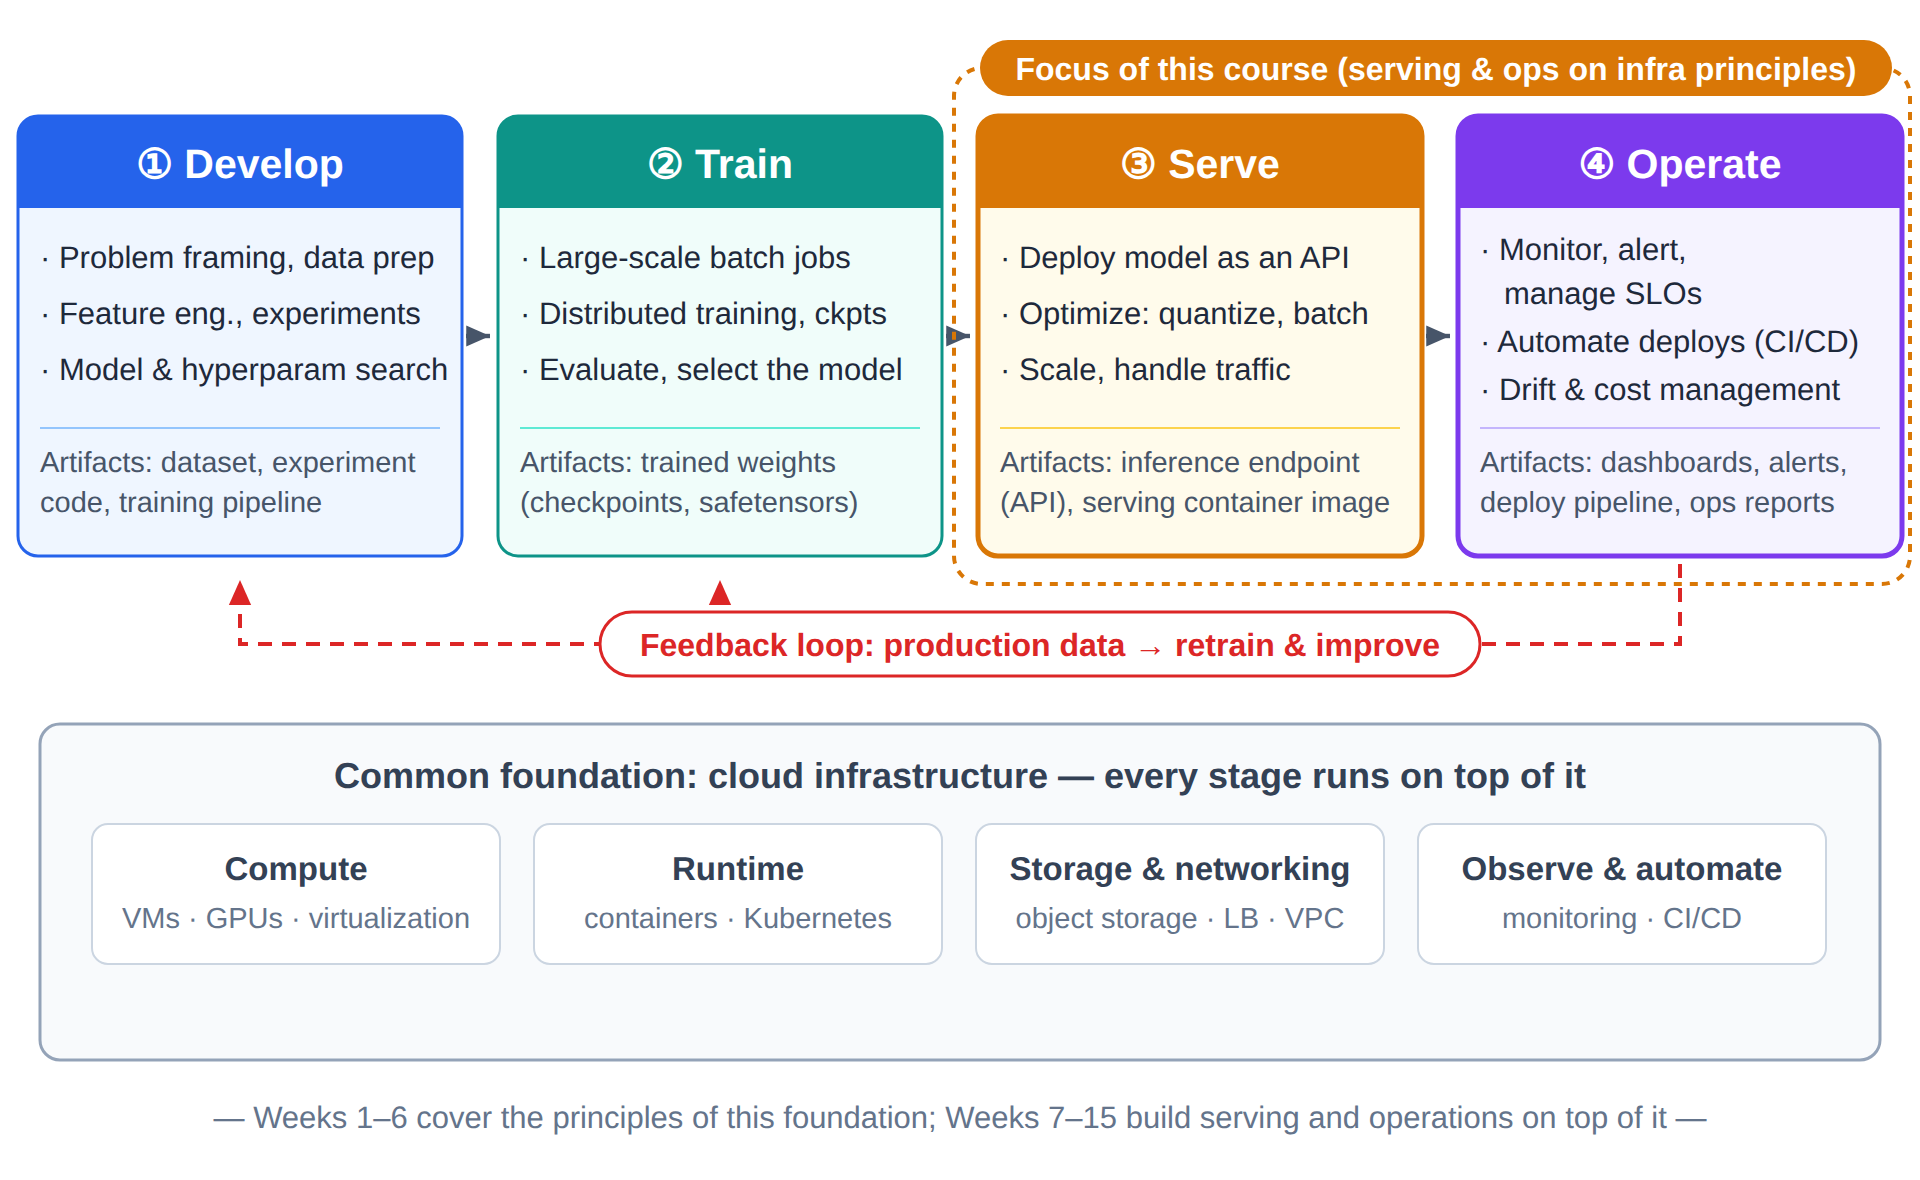
\includegraphics{figures/fig1-1_stack.png}}\\[3pt]
  \figcaption{Figure 1-1  The full AI service stack. The four stages form a loop connected by feedback, not a straight line — and every stage runs on cloud infrastructure.}
\end{tbbfigure}

\subsection*{A quick tour of the four stages}

In the \textbf{① development} stage you define the problem, collect and clean data, and experiment with model architectures and training recipes. The natural habitat is Jupyter notebooks and experiment trackers; from an infrastructure standpoint the usage pattern is interactive — small GPUs, used briefly and often. The artifacts are a curated dataset and a reproducible training pipeline.

In the \textbf{② training} stage you execute that pipeline for real. For large models this becomes distributed training across tens to thousands of GPUs running for days, with checkpoints saved along the way in case of failure. The artifact of this stage is the starting point of this course: \textbf{trained model weights} — in practice a file (checkpoints, \code{safetensors}, and so on) ranging from a few gigabytes to hundreds. Model formats are covered in Week 7.

In the \textbf{③ serving} stage that model file becomes a service handling real traffic. You wrap the model in an inference server and a container, deploy it to the cloud and expose it as an endpoint, manage latency and cost with optimizations such as quantization and batching, and adjust the number of instances as traffic changes. The entire middle of this course (Weeks 7–12) lives in this stage — it is where Exhibit A's team needed help.

The \textbf{④ operations} stage never ends while the service is alive. You continuously observe latency, throughput, error rates, and GPU utilization; you build automated pipelines that deploy new model versions safely; and you watch for \textbf{drift} — the quiet degradation that happens when the input distribution shifts away from what the model was trained on. This is the subject of Weeks 13–15.

The crucial point is that these four stages are \textbf{a cycle, not a waterfall.} User data and failure cases collected in operations flow back into development and training to produce the next model version, which then passes through serving again. The more mature the organization, the more automated and the faster this loop runs. The culture and tooling that make the loop spin well go by the name \textbf{MLOps}, the topic of Week 13.

\subsection*{Zooming into the serving stage}

Let us zoom into the stage this course centers on. Figure 1-2 traces the path of a single user request from arrival to response. The request first passes an API gateway and a load balancer — the component that, in Exhibit A, was the one returning 504s when the queue behind it outlasted its patience — where it is authenticated and dispatched to one of several serving \textbf{replicas}. Inside the replica, model execution is just one segment between preprocessing and postprocessing. The model weights were loaded at startup from a \textbf{model store built on object storage}, and a monitoring system collects metrics from every part of this path — giving the autoscaler the evidence it needs to adjust the number of replicas.

\begin{tbbfigure}
  \adjustbox{max width=0.94\linewidth,max totalheight=0.46\textheight}{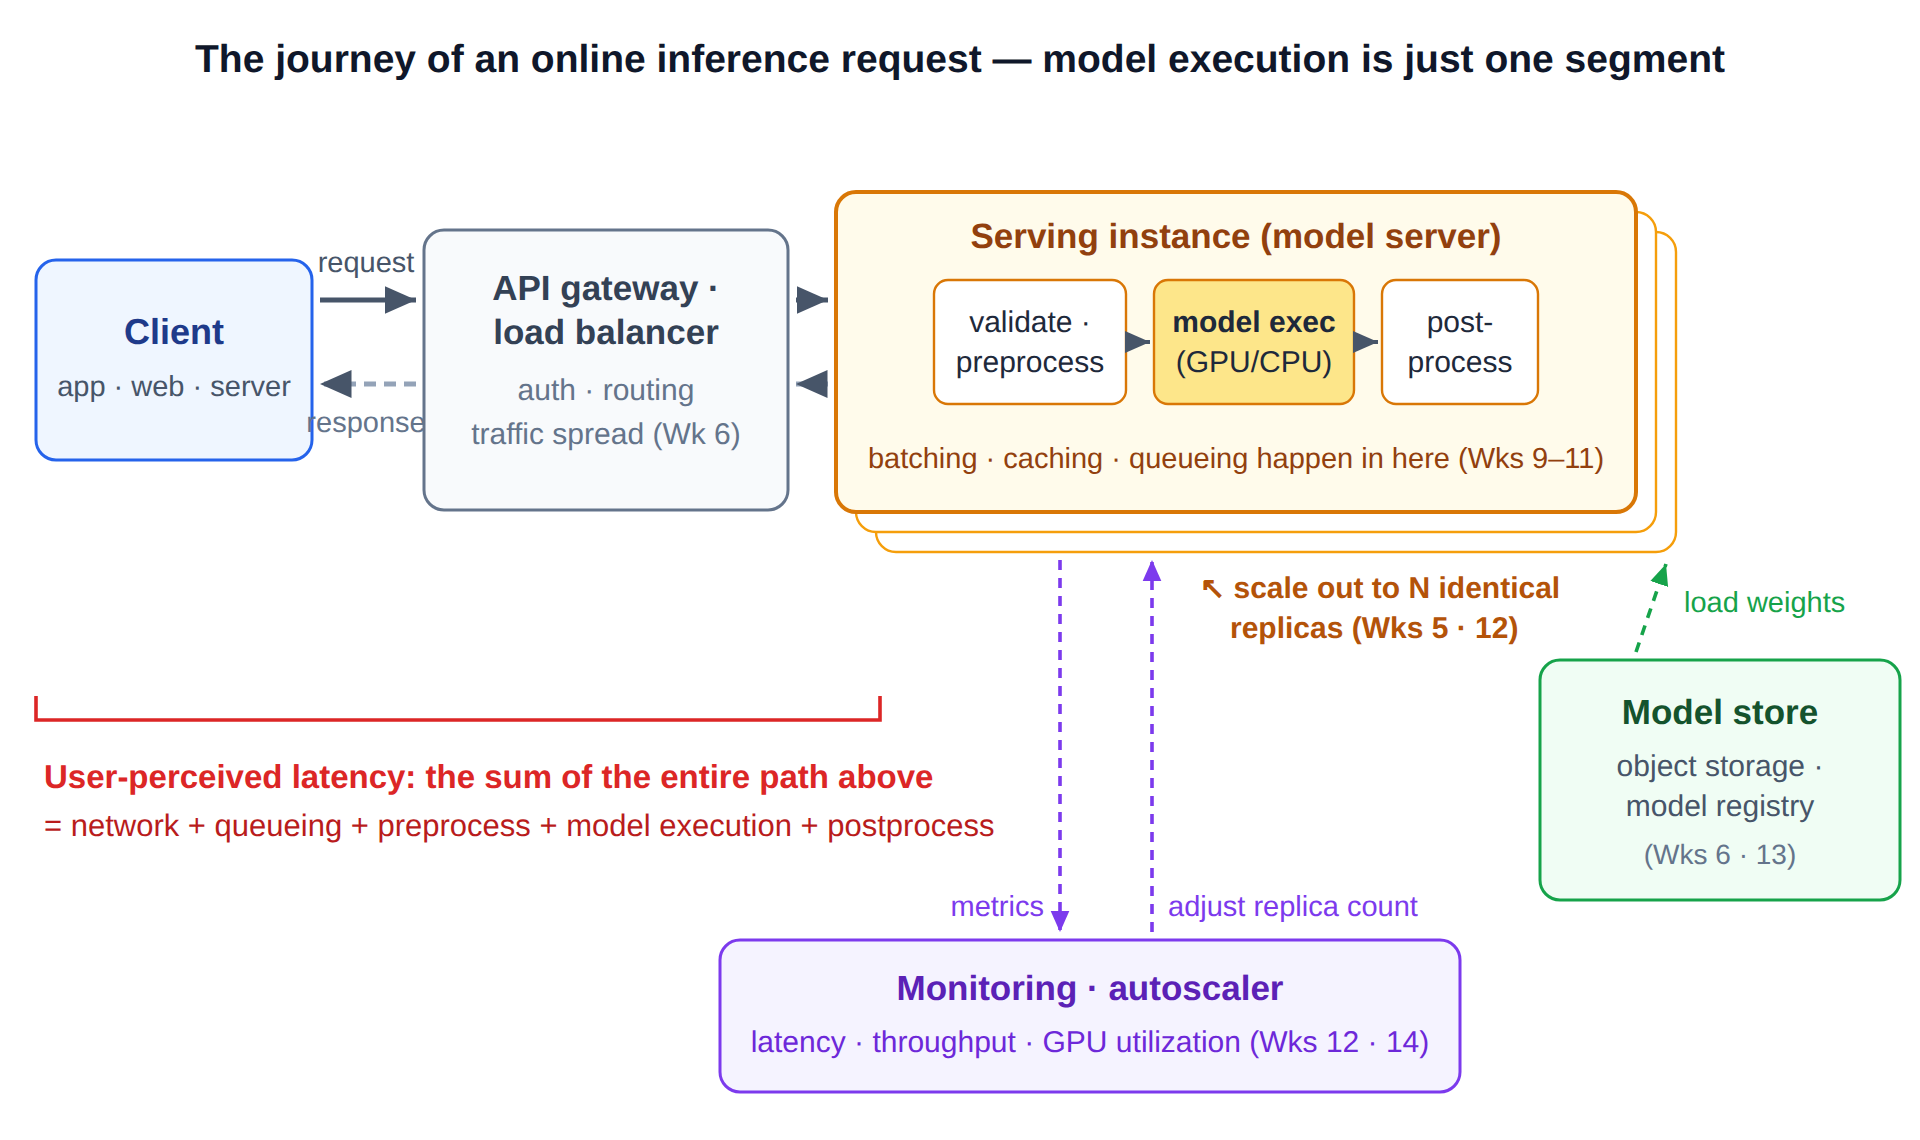
\includegraphics{figures/fig1-2_request_path.png}}\\[3pt]
  \figcaption{Figure 1-2  The journey of an online inference request. What the user feels as latency is the sum of the whole path, not the model execution time.}
\end{tbbfigure}

Two things in this figure are worth committing to memory. First, \textbf{user-perceived latency is the sum of the entire path.} If model execution takes 50 ms on the GPU but the request waited 2 seconds in a queue, the user experienced a slow service — full stop. Exhibit A was an extreme case: 0.31 s of model time inside a 30-second experience. Performance analysis in serving systems is therefore always the question, "which segment is the bottleneck?" Second, every component in this figure reappears somewhere in this course: the load balancer and object storage in Week 6, batching inside the serving replica in Weeks 9–11, the autoscaler in Week 12, monitoring in Week 14. You can treat Figure 1-2 as the map of this book.

\begin{calloutbox}{tbbpurple}{tbbpurplefill}
{\normalsize\bfseries\color{tbbpurple}Think About It}\par\vspace{3pt}
\begin{tbbitemize}
  \item In Figure 1-2, divide the latency segments into those you can control and those you mostly cannot. (Hint: who controls the user's network?)
  \item Why load model weights from object storage instead of baking them into the container image? What goes wrong when the model is 50 GB? (You will confirm the answer in Week 6.)
\end{tbbitemize}
\end{calloutbox}

\section{Training Workloads vs. Inference Workloads}

Even with the same GPU and the same model, "training" and "serving inference" are, from an infrastructure point of view, entirely different animals. Understanding this difference precisely is the most important goal of this chapter, because the design decisions that appear throughout the course — why serving scales out with many small instances, why autoscaling is non-negotiable, why GPU utilization is a headache — all originate here. Figure 1-3 lays out the contrast along six dimensions.

\begin{tbbfigure}
  \adjustbox{max width=0.94\linewidth,max totalheight=0.46\textheight}{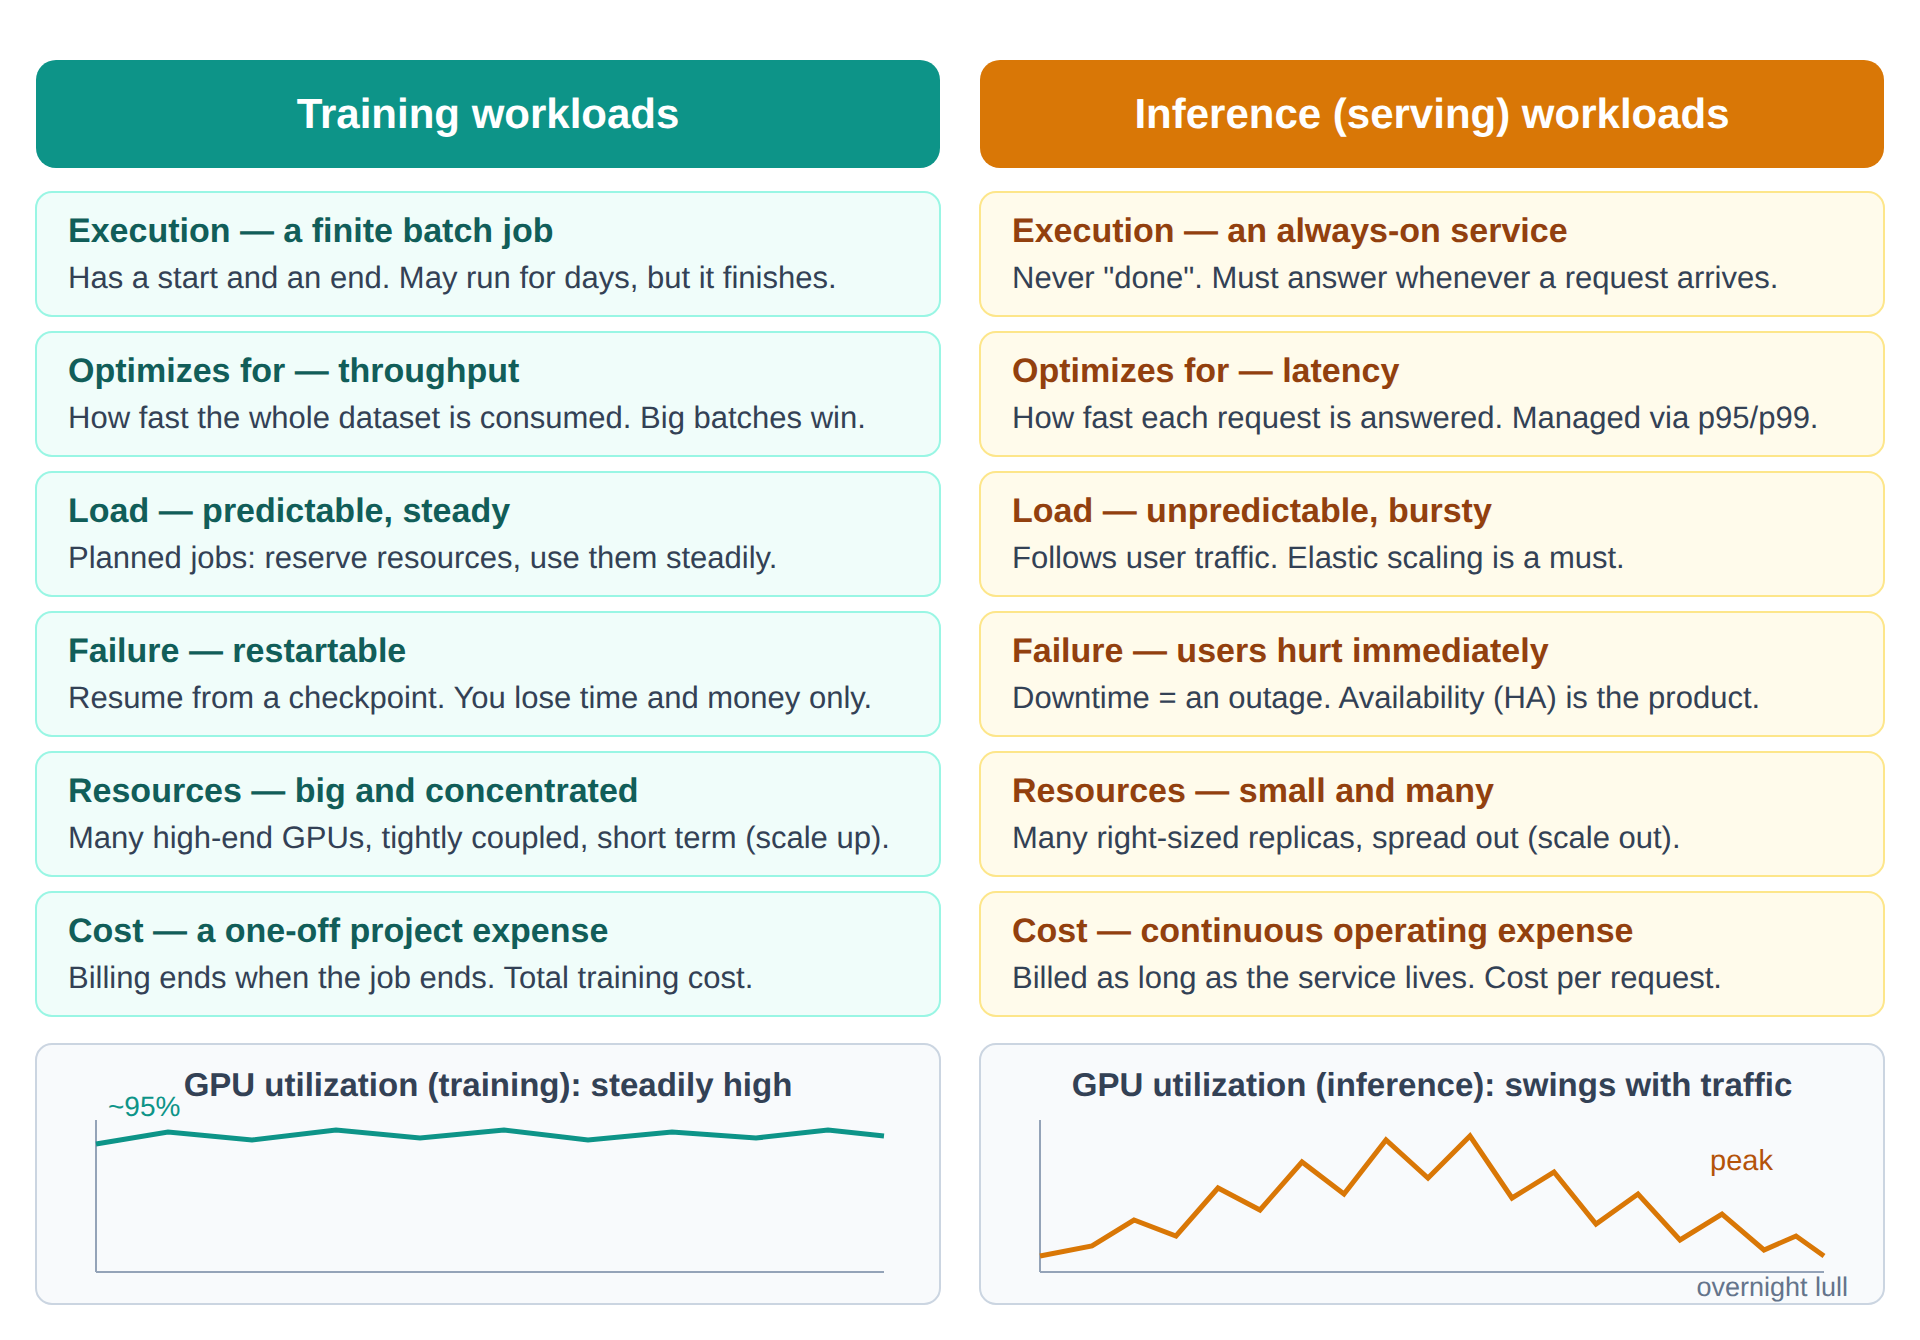
\includegraphics{figures/fig1-3_train_vs_infer.png}}\\[3pt]
  \figcaption{Figure 1-3  Training vs. inference workloads. The GPU-utilization contrast at the bottom foreshadows the autoscaling and GPU-sharing topics later in the course.}
\end{tbbfigure}

\subsection*{A job versus a service}

The most fundamental difference is the execution form. Training is \textbf{a batch job with a beginning and an end.} Whether it takes three days or three weeks, when it finishes it returns its resources. Serving is \textbf{an always-on service with no end}: it must stand ready to answer requests that may arrive at any moment. This difference reshapes the infrastructure. The key components of a training platform are a job queue and a batch scheduler; the key components of a serving platform are a load balancer, an orchestrator that guarantees the service keeps running (this is what a Kubernetes Deployment does — Week 5), and automatic recovery from failure. It is also why Exhibit B happened: a \textit{job} releases its machine when it ends; a \textit{service} has no end, so its machine has no default off-switch.

\subsection*{Throughput-oriented versus latency-oriented}

Training's performance metric is throughput: how many hours per epoch, how many samples per second. Whether an individual sample takes 0.1 s or 1 s is irrelevant as long as the whole run finishes sooner. Training therefore makes the \textbf{batch} — the group of samples the GPU processes at once — \textbf{as large as possible}, saturating the hardware.

Serving flips the metric to per-request latency, and a fundamental tension appears. From the GPU's point of view, gathering requests into bigger batches raises throughput and lowers cost; but the first request to arrive must \textbf{wait} for the batch to fill, so its latency suffers. This tug-of-war runs through all of serving-system design, and the techniques that resolve it cleverly — dynamic batching (Week 10) and continuous batching (Week 11) — are highlights of this course.

One more thing: in serving, latency is managed by the \textbf{tail}, not the average. If the mean response is 100 ms but one user in a hundred waits 5 seconds, then a service handling 100,000 requests a day delivers 1,000 bad experiences daily. Practitioners therefore set targets on p95 and p99 — the latency at the 95th and 99th percentile when all requests are sorted from fastest to slowest. "p99 ≤ 500 ms" is a promise: 99\% of requests are answered within half a second. Exhibit A's p99 was 30 seconds, set not by the model but by a queue; that is exactly why the tail, not the mean, is where service quality lives. Week 7 develops this into SLOs.

\subsection*{The serving triangle: latency, throughput, cost}

The batching tug-of-war is one instance of a pattern so central to this course that it deserves a name and a figure. Three things are wanted of every serving system: \textbf{low latency} (each user answered fast), \textbf{high throughput} (many users answered per second), and \textbf{low cost} (few dollars per answer). The engineering fact of life is that \textit{any two can be bought by spending the third} — and no trick buys all three at once. Figure 1-7 is the course's compass.

\begin{tbbfigure}
  \adjustbox{max width=0.94\linewidth,max totalheight=0.46\textheight}{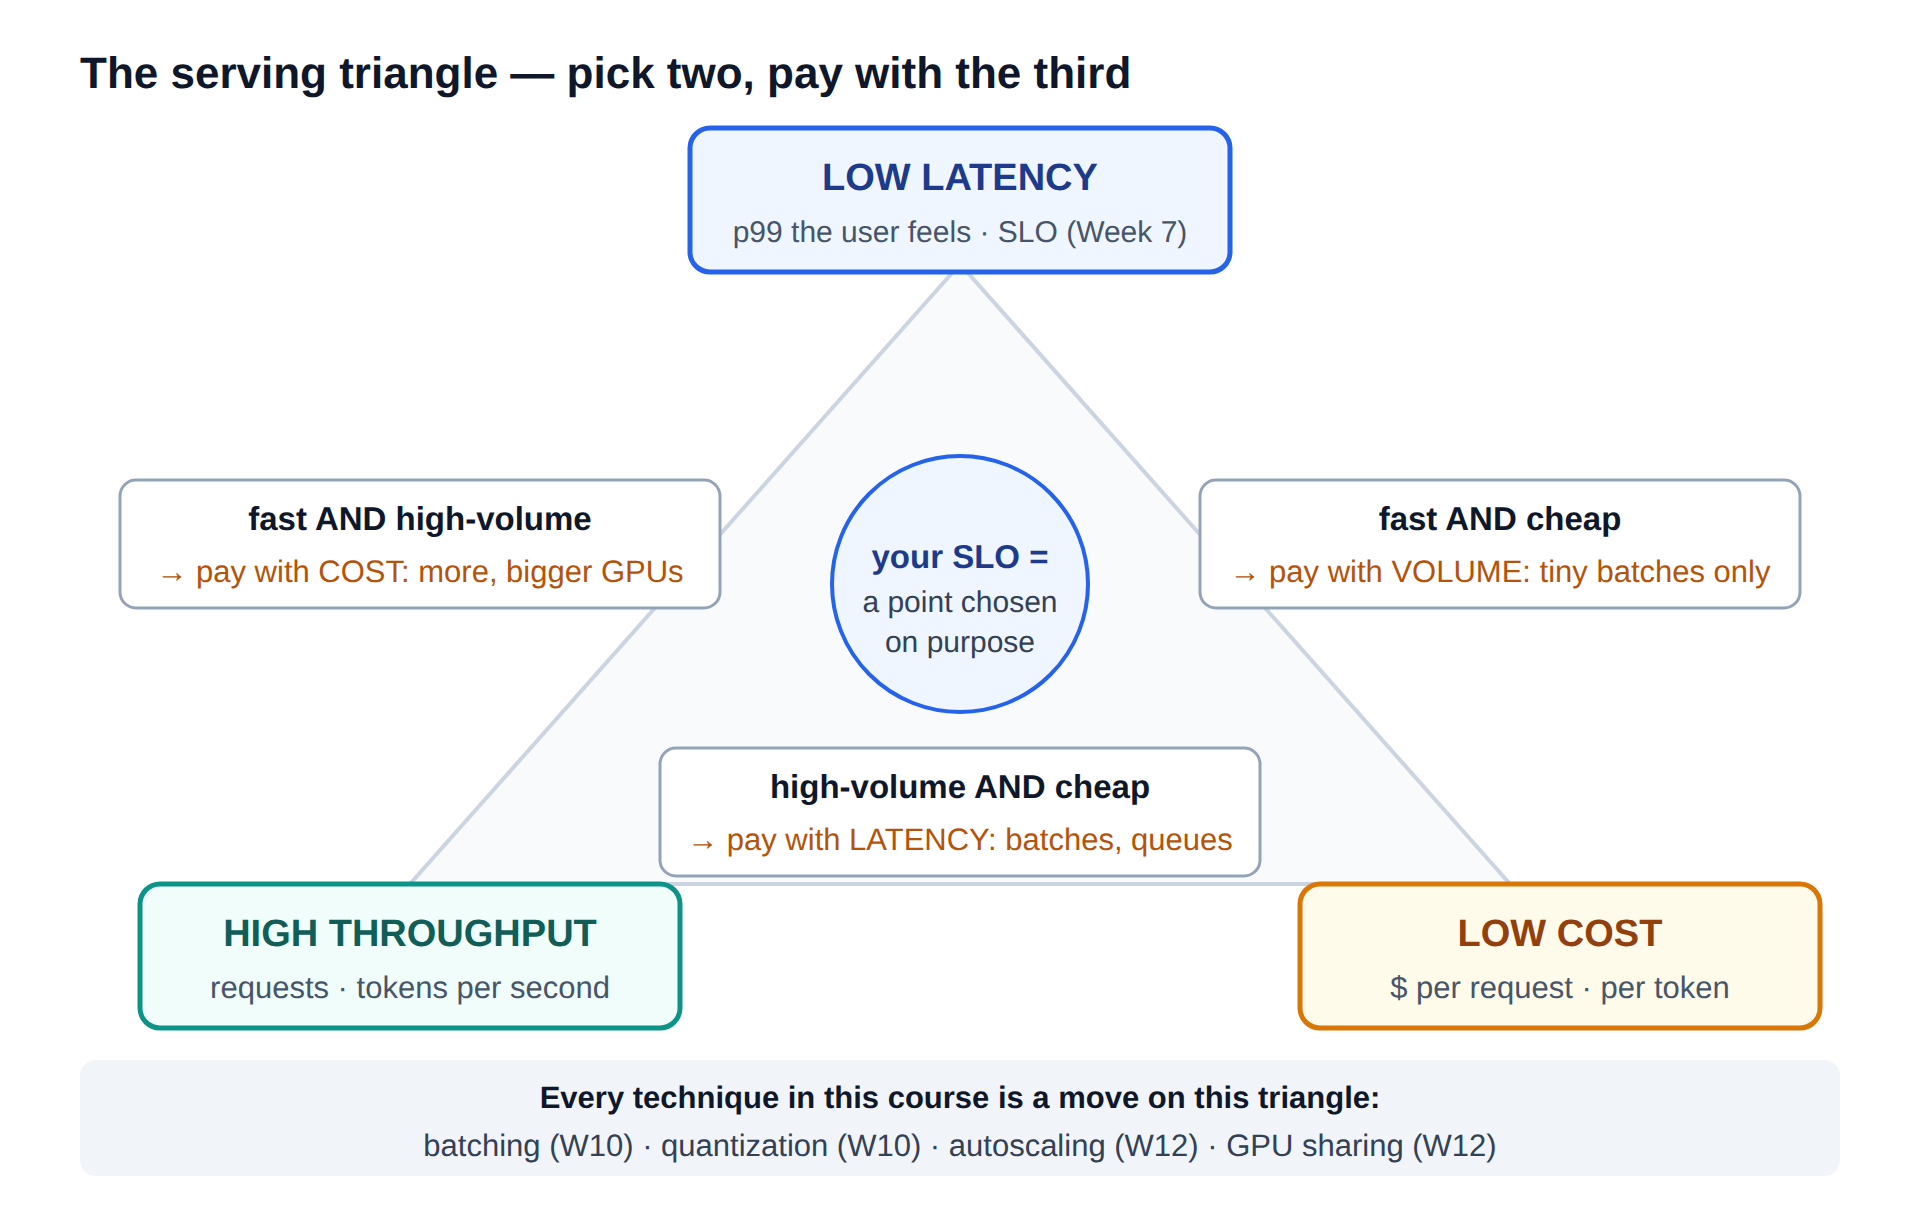
\includegraphics{figures/fig1-7_triangle.png}}\\[3pt]
  \figcaption{Figure 1-7  The serving triangle. Every optimization technique in this course is a move on this triangle — the discipline is naming what you pay before taking what you get.}
\end{tbbfigure}

Walk the three edges once. \textbf{Fast and high-volume} is easy: run many replicas, batch lightly, keep headroom everywhere — and pay with \textbf{cost} (Exhibit B is this corner's cautionary tale: capacity nobody used). \textbf{High-volume and cheap} is also easy: batch aggressively, run every GPU near saturation — and pay with \textbf{latency}, because full pipes mean queues, and queues live in the tail (Exhibit A, involuntarily). \textbf{Fast and cheap} works too — right up until volume arrives: one small warm instance answers its few requests instantly and inexpensively, and collapses the moment traffic grows. What is \textit{not} on the menu is all three corners at once at a fixed level of engineering skill. What this course teaches is, in one sentence, \textbf{how to move the whole triangle} — quantization (Week 10) makes each request cheaper \textit{and} faster; continuous batching (Week 11) buys throughput at less latency cost than naive batching; autoscaling (Week 12) rents the cost corner only when traffic needs it.

Two habits follow from the triangle, and they will be graded. First, \textbf{an SLO is a chosen point, not a wish}: "p99 ≤ 500 ms at 200 req/s under \$900/month" names a spot inside the triangle and commits to it — your team project's proposal (Week 7) does exactly this, and your Week 15 demo is measured against it. Second, \textbf{every optimization claim must name its payment}: "we made it faster" is not engineering until it continues "...at the price of X\% more GPU-hours" or "...by giving up batch sizes above 8." When a later chapter says \textit{read this with Chapter 1's cost lens}, this is the lens: which corner is being bought, which corner is paying, and is the exchange rate worth it?

\subsection*{Steady load versus bursty load}

A training job's load is predictable: the job I launched runs at the batch size I chose. A serving workload's load is decided by users. It surges at lunchtime, goes quiet overnight, and can jump tenfold on a marketing event or a viral post — Exhibit A's Discord message was a miniature viral post, and ChatGPT's launch was the full-sized version. This produces the classic dilemma of serving infrastructure: \textbf{provision for the peak and you waste money off-peak} (ten GPUs humming at 4 a.m. for a tenth of the traffic — Exhibit B at fleet scale); \textbf{provision for the average and the service collapses at the peak} (Exhibit A). The remedy is autoscaling — growing and shrinking resources with load — and its logical extreme is scale-to-zero: zero instances when there are no requests. But a GPU serving instance takes tens of seconds to minutes to come up (loading the model is the slow part). That is the \textbf{cold start} problem, and when we meet it in Week 12 we will reach back to the Firecracker microVMs of Week 2 for the solution.

\subsection*{The weight of failure}

If a GPU dies mid-training, it is annoying but not a disaster: resume from the last checkpoint. What is lost is time and money. A serving failure is different in kind — \textbf{the users on the service right now are harmed immediately.} They see error pages, or they stare at a spinner and leave. Serving systems are therefore obsessed with eliminating single points of failure: always run at least two replicas, replace dead instances automatically (Kubernetes' self-healing — Week 5), and roll new versions out gradually, shifting a small share of traffic first (canary deployment — Week 13).

\subsection*{The shape of resource use — including the shape in time}

Memory requirements differ at the root. Training must keep in GPU memory not only the weights but also the gradients, the optimizer state (twice the weights again, for Adam), and intermediate activations. Inference needs only the weights and the activations of the current requests. As a rule of thumb, inference needs roughly a third to a quarter of training's memory for the same model — and \textbf{quantization} (Week 10), which lowers the numeric precision of the weights, shrinks it further. This is why inference can run without the latest giant GPUs, and why this course's labs are designed to fit a single T4 or a Colab session.

But do not let "less memory" suggest "steady memory," because an inference server's memory use has a \textbf{shape in time}, and the shape is spiky. The weights are the flat baseline — loaded once, resident forever. On top of that baseline, every in-flight request allocates working memory for its activations, and that allotment scales with \textbf{how many requests are being processed at once (the batch) and how large each input is} (for LLMs: sequence length — and a per-request growing structure called the KV cache, the star of Week 11). A server that idles at 6 GB can spike well past 8 GB the moment a burst of long inputs arrives together. Now recall Exhibit A: bursts are precisely what production traffic does. This is why the folk sizing rule — \textit{watch the server idle for a day, add 10\%, set that as the memory limit} — is not caution but a scheduled outage: the limit will hold through every quiet hour and then execute your server at the first real burst, with a \code{137} in the logs (many stateless web apps, whose per-request footprint is a few kilobytes of strings, tolerate the same rule fine — that is why the habit exists and why it transfers so badly to inference). Week 3 gives the execution mechanism its real name — the cgroup and the OOM killer — and Chapter 3's exercises will ask you to explain this exact failure. You now can.

Hardware choices diverge too. Training is communication-heavy (gradient synchronization), so it favors clusters of high-end GPUs (H100, B200 class) stitched tightly together with NVLink and InfiniBand. Inference replicas barely talk to each other, so it is usually cheaper to scatter inexpensive inference GPUs (L4, T4) in many places — and small models are even served on CPUs with runtimes like \code{llama.cpp}, which is this course's fallback path if you have no GPU.

\begin{calloutbox}{tbbteal}{tbbtealfill}
{\normalsize\bfseries\color{tbbx115E59}Box 1-1  Why GPUs — and why an idle GPU is a problem}\par\vspace{3pt}
Deep learning computation is, at heart, enormous matrix multiplication, and matrix multiplication splits into thousands of small independent computations that can run at the same time. A GPU is hardware built to do exactly that, with thousands of cores. If a CPU is a few brilliant workers, a GPU is a brigade of thousands of simple ones.

The catch is price. A data-center GPU server costs several dollars per hour (Section 1.5). Training keeps its GPUs above 95\% busy and then releases them; an inference service that follows user traffic routinely sees average utilization fall to a few tens of percent or below — Exhibit B's 0.2\% is extreme only in degree. \textbf{An expensive resource sitting idle} — that is the essence of the AI serving cost problem, and batching (Week 10), GPU sharing and MIG (Weeks 2 · 12), autoscaling (Week 12), and spot instances (Week 12) are all attacks on it.
\end{calloutbox}

\vspace{3.0pt}

\subsection*{The shape of cost: one-off spend versus continuous spend}

Finally, cost structure. Training cost is project-shaped: "this training run took 400 GPU-hours, about X dollars" — paid once, then done. Serving cost is \textbf{an operating expense that recurs every month for as long as the service lives.} It grows with traffic, and it quietly balloons if neglected. Serving cost is therefore managed not as a total but as \textbf{cost per request} (or per token); that metric is both the success measure of optimization (Week 10) and a required deliverable of the team project (the monthly operating cost estimate).

One consequence of per-request costing deserves its own sentence, because Chapter 5 will lean on it: since the bill arrives per machine but value arrives per request, serving economics constantly plays a game called \textbf{density} — how many replicas can share one machine without hurting each other? Give each replica generous private headroom and you run few replicas per machine: safe, and expensive. Pack them tight and one replica's burst becomes its neighbor's latency spike. Every gigabyte of per-replica headroom is thus \textbf{a density/cost trade made on purpose}, and the tooling that makes the trade enforceable — resource requests and limits — is exactly what Chapters 3 and 5 build up to.

To summarize: every topic in the second half of this course is a corollary of this section's contrasts. Because serving is an always-on service, it needs orchestration and self-healing (Week 5); because it is latency-oriented, batching and optimization are hard and interesting (Weeks 10–11); because load is bursty, autoscaling and cold starts matter (Week 12); and because failure is heavy, deployment strategy and monitoring must be sophisticated (Weeks 13–14). Keep this sentence — and the triangle — as the summary of the chapter.

\begin{calloutbox}{tbbpurple}{tbbpurplefill}
{\normalsize\bfseries\color{tbbpurple}Think About It}\par\vspace{3pt}
\begin{tbbitemize}
  \item Consider a product-recommendation model for an online store. For its "training" and its "serving," sketch concrete numbers for each of the six dimensions in Figure 1-3. (When is peak traffic, for instance?)
  \item Place three services on the serving triangle: a free hobby project, a stock-trading signal API, and an overnight batch captioner for a photo archive. Which corner does each sacrifice — and which SLO number would each write down?
  \item Some inference does not need to happen live — e.g., classifying yesterday's photos overnight. Which column of Figure 1-3 does such "batch inference" resemble? What gets simpler in the infrastructure? (Preview of Week 7.)
\end{tbbitemize}
\end{calloutbox}

\section{Cloud Service Models and AI Infrastructure}

The traits of inference workloads we saw in the last section — bursty load, always-on operation, expensive GPUs — lead naturally to one question: \textbf{where should this infrastructure live, and how much of it should you manage yourself?} Exhibit B's team answered it by reflex ("rent one VM, install everything by hand") and paid \$779 for it; this section organizes the options they never considered.

\subsection*{Why the cloud}

Compared with buying and running your own GPU servers (on-premises), the cloud's advantages are especially pronounced for AI workloads. First, \textbf{capital expenditure becomes operating expenditure.} A data-center-grade GPU server costs tens to hundreds of thousands of dollars; in the cloud you rent it for a few dollars an hour and walk away when you are done. Second, \textbf{elasticity}: only a rented infrastructure can grow and shrink with the bursty inference load of Section 1.3. Third, \textbf{the risk of hardware generations is transferred.} New GPUs arrive every one to two years and old ones lose value fast; in the cloud you simply switch instance types. The cloud is not always the answer — an organization with permanently high utilization at large scale eventually finds ownership cheaper, and some data may not be allowed to leave the building. So the precise question is not "cloud or not" but "\textbf{up to which level do we rent?}"

\subsection*{The classic three layers: IaaS, PaaS, SaaS}

Cloud services are traditionally classified by how much the provider manages for you. \textbf{IaaS} (Infrastructure as a Service) rents you the raw materials — virtual machines, storage, networks — and everything above the OS is your problem. \textbf{PaaS} (Platform as a Service) manages the runtime platform too, so you bring only your application. \textbf{SaaS} (Software as a Service) is finished software you simply use. The lower you go, the more control; the higher you go, the less there is to operate.

AI infrastructure inherits these three layers and inserts finer gradations between them. Figure 1-4 shows the spectrum.

\begin{tbbfigure}
  \adjustbox{max width=0.94\linewidth,max totalheight=0.46\textheight}{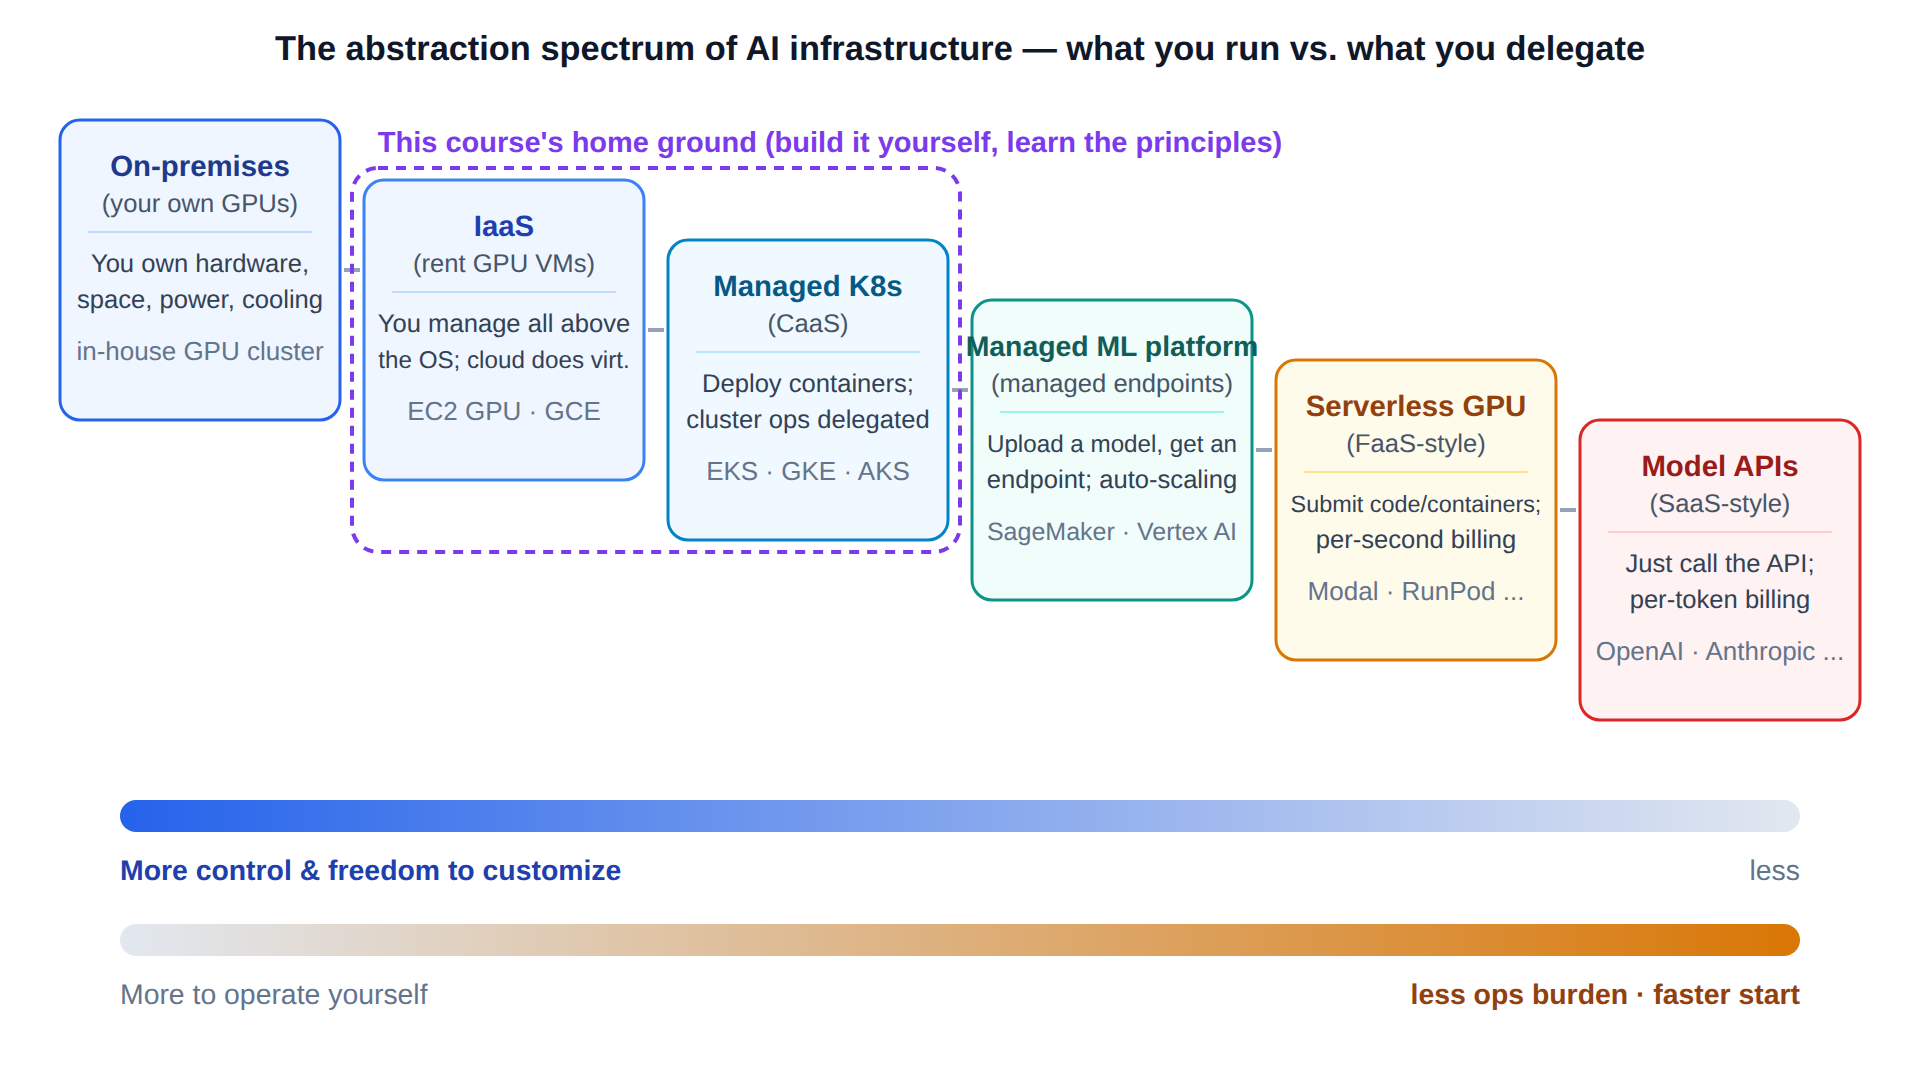
\includegraphics{figures/fig1-4_abstraction.png}}\\[3pt]
  \figcaption{Figure 1-4  The abstraction spectrum of AI infrastructure. Rightward means less to operate but also less control. This course works — deliberately — in the IaaS-to-managed-K8s range.}
\end{tbbfigure}

Read the steps from a serving perspective. A \textbf{GPU VM (IaaS)} rents you a whole machine with a GPU attached: you can do anything, and you must do everything, from OS patches to failure recovery. \textbf{Managed Kubernetes (CaaS)} rents you a container-orchestration cluster: deployment, scaling, and recovery of containers are handled by the platform. It is the de facto standard for self-managed serving today and the home ground of this course (Week 5). A \textbf{managed ML platform} (SageMaker, Vertex AI, and friends) rises to "hand us a model file, receive an endpoint" (introduced in Week 13). A \textbf{serverless GPU} platform takes just a container or function and allocates a GPU only while requests are being handled, billing by the second — Exhibit B mathematically cannot happen there, in exchange for cold starts (Week 12). At the far right, a \textbf{model API} means using someone else's model on someone else's infrastructure and paying per token: SaaS-style consumption of AI.

\begin{tbbtablewrap}
  \begin{tabular}{@{}>{\raggedright\arraybackslash}m{\dimexpr 0.2021\tbltextwidth-2\tabcolsep\relax} >{\raggedright\arraybackslash}m{\dimexpr 0.2660\tbltextwidth-2\tabcolsep\relax} >{\raggedright\arraybackslash}m{\dimexpr 0.2766\tbltextwidth-2\tabcolsep\relax} >{\raggedright\arraybackslash}m{\dimexpr 0.2553\tbltextwidth-2\tabcolsep\relax}@{}}
  \arrayrulecolor{tbbnavy}\specialrule{1pt}{0pt}{0pt}
  \rowcolor{tbbtablehead}{\centering \bfseries\color{tbbnavy}Layer} & {\centering \bfseries\color{tbbnavy}What you rent} & {\centering \bfseries\color{tbbnavy}What you still manage} & {\centering \bfseries\color{tbbnavy}Serving example} \\
  \arrayrulecolor{tbbnavy}\specialrule{0.7pt}{0pt}{2pt}
  {\textbf{IaaS}} & {GPU VMs, storage, network} & {OS, runtime, serving SW, scaling, recovery} & {Install vLLM directly on an EC2/GCE GPU instance} \\
  \arrayrulecolor{tbbtableborder}\hline
  {\textbf{CaaS}} & {+ K8s cluster operation} & {Container images, deployment specs, serving config} & {Model server on EKS · GKE (this course)} \\
  \arrayrulecolor{tbbtableborder}\hline
  {\textbf{PaaS / ML platform}} & {+ serving runtime, scaling, deploys} & {Model artifact, configuration} & {SageMaker · Vertex AI endpoints} \\
  \arrayrulecolor{tbbtableborder}\hline
  {\textbf{Serverless GPU}} & {+ the entire instance lifecycle} & {Container/function code} & {Modal, RunPod Serverless, ...} \\
  \arrayrulecolor{tbbtableborder}\hline
  {\textbf{SaaS (model API)}} & {Model and infrastructure, all of it} & {Prompts, calling code} & {OpenAI, Anthropic, etc. model APIs} \\
  \arrayrulecolor{tbbnavy}\specialrule{1pt}{2pt}{0pt}
  \end{tabular}\par
  \figcaption{Table 1-2  Serving at each service level: what you rent vs. what you manage}
\end{tbbtablewrap}

Let us also be explicit about this course's pedagogical choice. In industry, picking the lower rows of the table (more abstraction) is often the sensible move. This course nevertheless walks the IaaS-to-CaaS road and \textbf{builds things by hand}, because when something breaks at a high abstraction level, the person who knows what is happening underneath responds in a completely different way from the person who does not. Reading a managed endpoint's bill, or shaving a serverless platform's cold start, ends up demanding an understanding of the layers below. Build it from the ground once, and no abstraction will make you nervous again.

\begin{calloutbox}{tbbpurple}{tbbpurplefill}
{\normalsize\bfseries\color{tbbpurple}Think About It}\par\vspace{3pt}
\begin{tbbitemize}
  \item You are building a campus chatbot whose traffic spikes only during course-registration week. Which point on Figure 1-4 would you choose? Argue in terms of idle cost and available operations staff.
  \item Look up the phrase "shared responsibility model." When a security incident happens on managed K8s, which parts are the provider's responsibility and which are yours?
\end{tbbitemize}
\end{calloutbox}

\section{The GPUaaS and Model-API Ecosystem}

Now to the actual market. In the past few years an ecosystem has grown explosively between two poles: \textbf{GPUaaS} (GPU-as-a-Service), which sells raw GPU compute, and \textbf{model APIs}, which sell model capability itself. The goal of this section is not to memorize company names — the market moves fast — but to acquire \textbf{a way of reading the terrain.}

\subsection*{Hardware sense: data-center GPUs}

Before the market, the merchandise. NVIDIA is the de facto standard for data-center GPUs, and each generation grows not just faster but bigger in \textbf{memory}: A100 (40/80 GB) → H100 (80 GB) → H200 (141 GB) → the Blackwell-generation B200 (192 GB), plus rack-scale systems like the GB200 NVL72 that fuse many CPUs and GPUs into one unit. Why does memory matter so much for serving? Because \textbf{the model must fit into GPU memory for inference to run at all.} A 70-billion-parameter model at 16-bit precision needs about 140 GB for weights alone — it does not fit on a single 80 GB H100. You must either shrink it by quantization (Week 10) or shard it across GPUs. Meanwhile, inference-oriented GPUs — L4 (24 GB), T4 (16 GB) — are cheap, low-power workhorses, and this course's labs are designed around a single T4.

This is also the first appearance of a sizing discipline the course will repeat until it is reflex: \textbf{find the binding dimension first.} For most inference, the constraint that binds is memory capacity (does the model fit?) or memory bandwidth (how fast can weights stream through the compute units?), not raw FLOPs — which is why a modest L4 often serves a small model at nearly the experience of an H100 at a fraction of the price, and why paying for the biggest GPU "to be safe" is usually paying for a dimension that was never the constraint. Instance choice should follow the binding dimension; every later cost exercise in this course (Weeks 9, 10, 12) starts there.

\begin{tbbtablewrap}
  \begin{tabular}{@{}>{\raggedright\arraybackslash}m{\dimexpr 0.3830\tbltextwidth-2\tabcolsep\relax} >{\raggedright\arraybackslash}m{\dimexpr 0.2553\tbltextwidth-2\tabcolsep\relax} >{\raggedright\arraybackslash}m{\dimexpr 0.3617\tbltextwidth-2\tabcolsep\relax}@{}}
  \arrayrulecolor{tbbnavy}\specialrule{1pt}{0pt}{0pt}
  \rowcolor{tbbtablehead}{\centering \bfseries\color{tbbnavy}Where you rent} & {\centering \bfseries\color{tbbnavy}Rough price band} & {\centering \bfseries\color{tbbnavy}Note} \\
  \arrayrulecolor{tbbnavy}\specialrule{0.7pt}{0pt}{2pt}
  {Hyperscalers (AWS · GCP · Azure)} & {\$3–7 / hour} & {A premium, in exchange for ecosystem integration} \\
  \arrayrulecolor{tbbtableborder}\hline
  {GPU-specialist clouds (Lambda, CoreWeave, ...)} & {\$2.0–2.5 / hour} & {Specialization keeps unit prices down} \\
  \arrayrulecolor{tbbtableborder}\hline
  {Marketplaces (Vast.ai, ...)} & {\$1.9–3.5 / hour} & {Brokered idle GPUs; cheap but variable} \\
  \arrayrulecolor{tbbtableborder}\hline
  {\textcolor{tbbgray}{(Reference) B200}} & {\textcolor{tbbgray}{\$4–6 / hour}} & {\textcolor{tbbgray}{Next generation, higher throughput}} \\
  \arrayrulecolor{tbbnavy}\specialrule{1pt}{2pt}{0pt}
  \end{tabular}\par
  \figcaption{Table 1-3  Rough hourly prices for an H100 (80 GB), on-demand, as of mid-2026}
\end{tbbtablewrap}

\begin{calloutbox}{tbbred}{tbbxFEF2F2}
{\normalsize\bfseries\color{tbbx991B1B}Warning: remember the structure, not the numbers}\par\vspace{3pt}
The numbers in this table will already be wrong by the time you read it — GPU prices move with generations and supply. What to remember is the structure: \textbf{① specialist clouds undercut hyperscalers on GPU price; ② the same GPU varies severalfold across committed-use, spot, and marketplace channels; ③ the meter runs by the hour, so idle time is money.} This is also why setting a billing alert is the very first lab task (Week 2).
\end{calloutbox}

\vspace{3.0pt}

\subsection*{A map of the ecosystem: six clusters}

Figure 1-5 arranges the ecosystem along one axis — "sells infrastructure" versus "sells model capability" — in six clusters.

\begin{tbbfigure}
  \adjustbox{max width=0.94\linewidth,max totalheight=0.46\textheight}{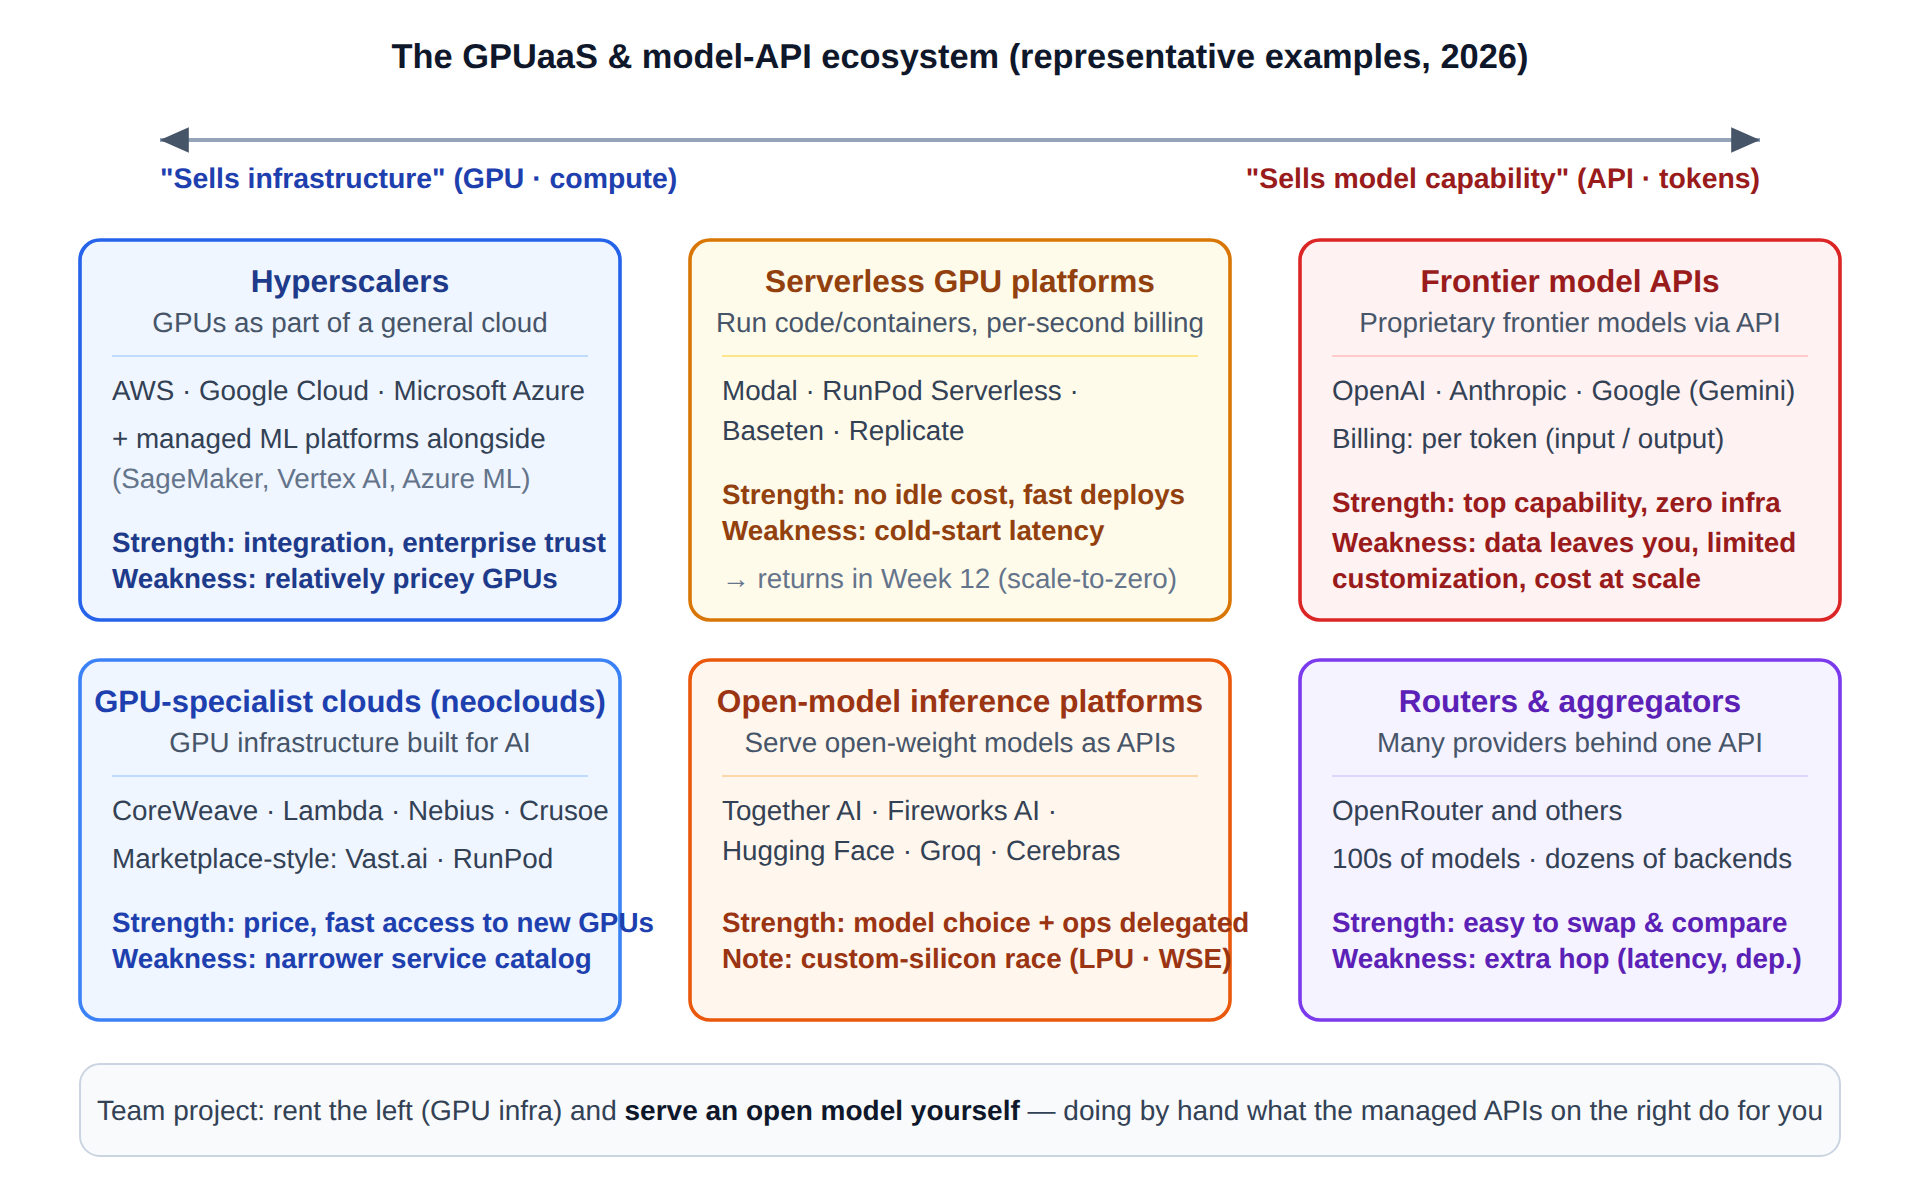
\includegraphics{figures/fig1-5_ecosystem.png}}\\[3pt]
  \figcaption{Figure 1-5  The GPUaaS and model-API ecosystem. Left sells compute; right sells capability. The company names are 2026 examples — the cluster boundaries are what matters.}
\end{tbbfigure}

\textbf{Hyperscalers} (AWS, Google Cloud, Azure) sell GPUs as one part of a general-purpose cloud, bundled with managed ML platforms. Their strengths are integration with everything else you run and mature security and compliance; their GPUs carry a premium. \textbf{GPU-specialist clouds} — the market calls them \textit{neoclouds} — are clouds built specifically for AI workloads: CoreWeave, Lambda, Nebius, Crusoe are representative. They adopt new GPUs quickly and price aggressively. Marketplace-style players such as Vast.ai broker idle GPUs — cheapest of all, if you accept variability in the supply.

\textbf{Serverless GPU platforms} (Modal, RunPod Serverless, Baseten, Replicate, ...) hide the very notion of a server and rent GPUs per invocation of your code or container. With billing only while requests run, they are attractive for spiky or low traffic — their weakness is the cold start we met in Section 1.3. \textbf{Open-model inference platforms} (Together AI, Fireworks AI, Hugging Face, ...) serve publicly released open-weight models behind an API — a middle ground offering the model freedom of self-serving with the operational ease of an API. In this cluster, companies like Groq (LPU) and Cerebras (WSE) compete on speed with custom non-GPU silicon. Finally, \textbf{frontier model APIs} (OpenAI, Anthropic, Google) sell closed frontier models per token, and \textbf{routers/aggregators} (OpenRouter and others) bundle all of the above behind a single API.

The most consequential trend reshaping this terrain in recent years is \textbf{the rise of open-weight models.} As the quality of models whose weights are publicly downloadable — the Llama, Qwen, DeepSeek, and Mistral families — has chased down the closed models, "serve a good model on my own infrastructure" has become a realistic option. As self-serving demand grows, the left side (GPU infrastructure) and the middle (serving technology) of the map grow with it — and that serving technology is exactly what this course teaches.

\subsection*{The machinery of the economy: keys, meters, and quotas}

Whichever cluster you buy from, the purchase itself has a common shape, and it is worth naming because this course will eventually make you build it. Every model API and GPU platform hands you an \textbf{API key} (identity: \textit{who} is calling), runs a \textbf{meter} (billing: per token, per second, per request), and encloses you in \textbf{quotas and rate limits} (protection: a ceiling on requests or tokens per minute, per tier). Exceed the ceiling and you receive HTTP \textbf{429 Too Many Requests} — not an outage, not an error in your code, but the provider's load balancer declining, politely and by design, to let your traffic hurt other tenants. Free tiers, usage dashboards, spend alerts, tiered pricing: all of it is the same three-part machinery of key, meter, and fence.

Why belabor something so mundane? Because the machinery is the product. The model answers requests, but the key–meter–quota apparatus is what makes answering requests \textit{a business} — it is how a fleet of GPUs someone else operates becomes a line item you can budget. And here is the loop this course will close: when you self-serve, \textbf{you become the provider}, and every piece reappears as your responsibility — the API gateway that checks keys and enforces limits is Week 6, the metering that tells you your own cost per token is Week 12, and your team project must expose its model behind exactly this kind of front door. By Week 6 you will be standing on the other side of this counter.

\subsection*{Build or buy: model API vs. self-serving}

The two ends of the ecosystem converge, in practice, on a single decision: \textbf{buy a model API, or build with an open model served by your own hands?} Table 1-4 collects the criteria.

\begin{tbbtablewrap}
  \begin{tabular}{@{}>{\raggedright\arraybackslash}m{\dimexpr 0.1915\tbltextwidth-2\tabcolsep\relax} >{\raggedright\arraybackslash}m{\dimexpr 0.4043\tbltextwidth-2\tabcolsep\relax} >{\raggedright\arraybackslash}m{\dimexpr 0.4043\tbltextwidth-2\tabcolsep\relax}@{}}
  \arrayrulecolor{tbbnavy}\specialrule{1pt}{0pt}{0pt}
  \rowcolor{tbbtablehead}{\centering \bfseries\color{tbbnavy}Criterion} & {\centering \bfseries\color{tbbnavy}Model API favored (buy)} & {\centering \bfseries\color{tbbnavy}Self-serving favored (build)} \\
  \arrayrulecolor{tbbnavy}\specialrule{0.7pt}{0pt}{2pt}
  {\textbf{Scale / traffic}} & {Small or uncertain — pay only for what you use} & {Large and steady — you can keep GPUs saturated} \\
  \arrayrulecolor{tbbtableborder}\hline
  {\textbf{Data / regulation}} & {No constraints on data leaving your boundary} & {Sensitive data; on-premises or data-sovereignty requirements} \\
  \arrayrulecolor{tbbtableborder}\hline
  {\textbf{Customization}} & {Generic capability suffices} & {Fine-tuned models, special domains, full control of outputs} \\
  \arrayrulecolor{tbbtableborder}\hline
  {\textbf{Latency control}} & {Provider SLAs are good enough} & {You must tune tail latency, batching, and hardware yourself} \\
  \arrayrulecolor{tbbtableborder}\hline
  {\textbf{Team capability}} & {No infrastructure engineers available} & {Engineers who took this course are available} \\
  \arrayrulecolor{tbbtableborder}\hline
  {\textbf{Peak capability}} & {You truly need frontier-class ability} & {Open-model quality is sufficient for the task} \\
  \arrayrulecolor{tbbnavy}\specialrule{1pt}{2pt}{0pt}
  \end{tabular}\par
  \figcaption{Table 1-4  Model API vs. self-serving: decision criteria}
\end{tbbtablewrap}

The cost axis yields to a quick back-of-envelope estimate — the numbers below are \textbf{hypothetical}. Suppose a service generates 20 million tokens a day with a small open model. Through an API priced at \$0.5 per million tokens, that is \$10 a day, roughly \textbf{\$300 a month}. Self-serving the same load on one L4 GPU at \$0.8/hour costs about \textbf{\$580 a month} always-on — \textbf{at this scale the API is cheaper.} Now let traffic grow twentyfold. The API bill scales linearly to \$6,000; the self-served cluster follows with just a few more GPUs, because batching pushes throughput up superlinearly (Week 10). Somewhere in between, the curves cross. Finding that break-even point properly requires GPU utilization, the level of optimization, and operations headcount — which is precisely the exercise your team project's "monthly operating cost estimate" asks you to do.

One final emphasis: this is not a binary choice. Real organizations commonly run a \textbf{hybrid strategy} — prototype and validate on a frontier API, then move the proven, high-traffic core onto self-served open models. Whichever side you pick, the goal of this section is that you pick it \textbf{knowing what you are giving up and what you are getting.}

\begin{calloutbox}{tbbpurple}{tbbpurplefill}
{\normalsize\bfseries\color{tbbpurple}Think About It}\par\vspace{3pt}
\begin{tbbitemize}
  \item A hospital wants an AI that summarizes clinical notes. Apply the criteria of Table 1-4: which criterion is the deal-breaker?
  \item In the back-of-envelope example, suppose the self-served GPU is only 30\% utilized (idle most of the day). What happens to the true cost per token? What are the ways to raise utilization? (Preview of Week 12.)
  \item You receive a 429 from a model API during your own service's traffic spike. Trace the irony: which part of the provider's key–meter–quota machinery just protected \textit{their} p99 at the cost of \textit{yours} — and what does that tell you about the SLO your service can promise while it depends on theirs?
\end{tbbitemize}
\end{calloutbox}

\section{Course Roadmap and How to Study}

Let us see how the big picture drawn in this chapter unfolds over the fifteen weeks ahead. Figure 1-6 is the full roadmap.

\begin{tbbfigure}
  \adjustbox{max width=0.94\linewidth,max totalheight=0.46\textheight}{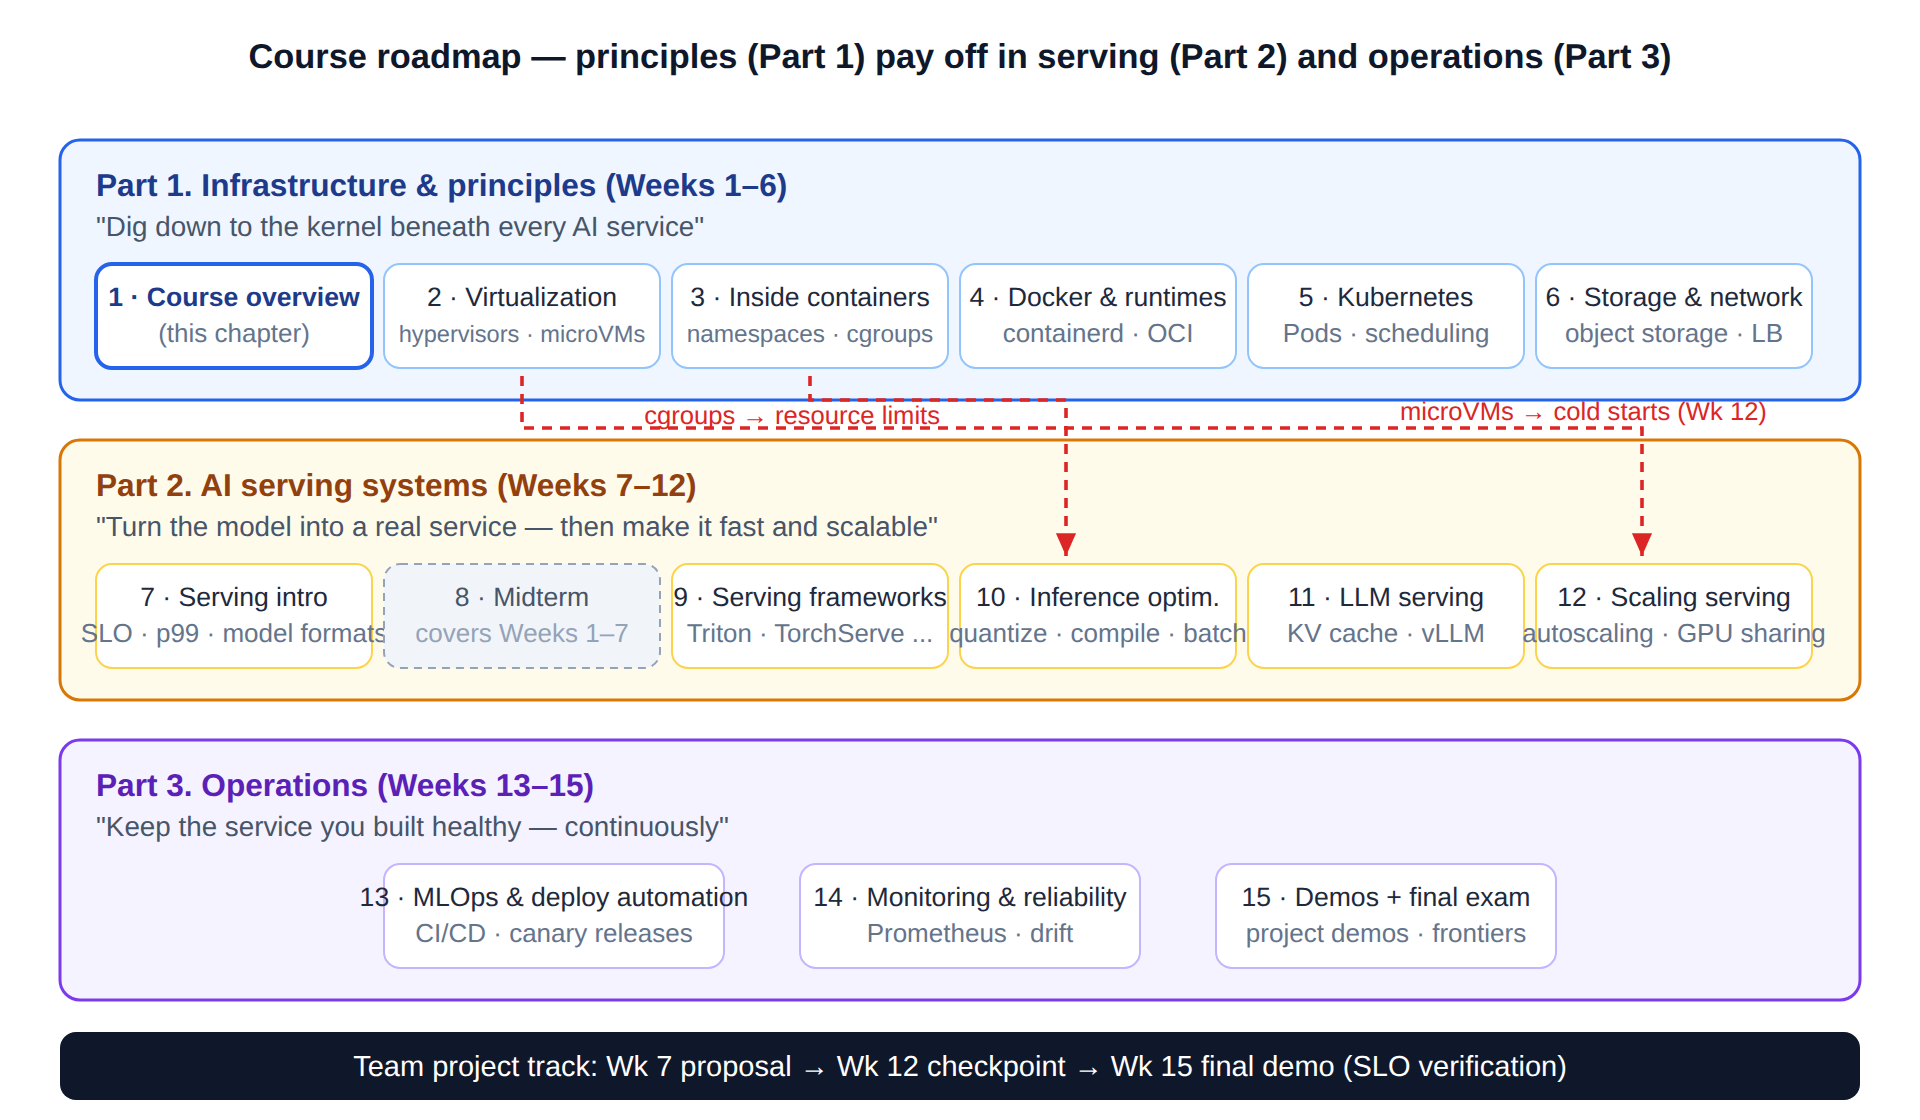
\includegraphics{figures/fig1-6_roadmap.png}}\\[3pt]
  \figcaption{Figure 1-6  The 15-week roadmap. The red dashed lines mark representative paths where Part 1 principles are "called back" by later topics.}
\end{tbbfigure}

\textbf{Part 1 (Weeks 1–6)} digs down to the kernel beneath the ground every AI service stands on: how virtualization works at the CPU-instruction level (Week 2), which kernel features a container is actually made of (Week 3), how Docker and Kubernetes package those features (Weeks 4–5), and what the storage and networks that carry model files and traffic look like (Week 6). \textbf{Part 2 (Weeks 7–12)} builds serving systems on that ground: the performance language of serving — SLOs, p99 (Week 7); serving a real model with a framework and load-testing it (Week 9); making it fast with quantization, compilation, and batching (Week 10); the peculiar world of LLM serving (Week 11); and scaling and cost (Week 12). \textbf{Part 3 (Weeks 13–15)} is operations: deployment automation (Week 13), monitoring and reliability (Week 14), and the team project finale (Week 15).

What the roadmap emphasizes is the red dashed lines — the \textbf{callback structure.} The first half of this course is foreshadowing for the second half, and it is deliberate enough that you will collect a pocketful of recurring souvenirs along the way. A partial list, so you can enjoy recognizing them when they arrive:

\begin{tbbitemize}
  \item \textbf{The number 137} — first met in this chapter as a cryptic exit code, inflicted on your own process in Week 3 (it is the kernel's OOM killer: 128 + SIGKILL's 9), enforced by Kubernetes in Week 5, and stalking every memory-sizing decision you make thereafter.
  \item \textbf{A mysterious parent process, PID 41288} — appears unexplained in Week 3's very first transcript when you start a container, and is finally interrogated and identified in Week 4. (No spoilers.)
  \item \textbf{A shipping container from 1956} — Week 4 opens with the story of how one steel box collapsed the cost of moving goods by \textasciitilde{}37×, and why Docker images are the same trick played on software. You will not look at the word "container" the same way again.
  \item \textbf{The Firecracker microVM of Week 2} (a VM that boots in milliseconds) returns in Week 12 when we discuss \textbf{GPU cold starts} — to answer "why is the first request slow on serverless GPUs," you need to know what it physically means for a machine to boot.
  \item \textbf{The cgroup files you write by hand in Week 3} (\code{memory.max}, \code{cpu.max}) are exactly where Kubernetes' resource requests/limits land in Week 5 — one mechanism wearing two interfaces, and the direct answer to this chapter's density/cost trade.
  \item \textbf{GPU virtualization in Week 2} (PCIe passthrough, vGPU, MIG) is called back in Week 12 as the \textbf{GPU sharing} strategy — how several services split one expensive GPU — after Week 4 explains why the kernel itself refuses to referee GPU time.
\end{tbbitemize}

\subsection*{The team project: this course's comprehensive exam}

The largest share of your grade (30\%) is the team project, and its assignment fits in one sentence: \textbf{"Pick an open-source AI model, deploy it to the cloud, and prove with a load test that it meets a target SLO."} Container-based serving on Kubernetes, autoscaling with SLO verification under load, a monitoring dashboard, a before/after optimization comparison, and a monthly operating-cost estimate — every topic this chapter toured appears in one project. The proposal is due in Week 7, the checkpoint in Week 12, the final demo in Week 15. This week's task is simply to form teams. The project is designed to be assembled from what each week teaches, so there is no reason to be intimidated now.

\begin{tbbtablewrap}
  \begin{tabular}{@{}>{\raggedright\arraybackslash}m{\dimexpr 0.2553\tbltextwidth-2\tabcolsep\relax} >{\raggedright\arraybackslash}m{\dimexpr 0.1489\tbltextwidth-2\tabcolsep\relax} >{\raggedright\arraybackslash}m{\dimexpr 0.5957\tbltextwidth-2\tabcolsep\relax}@{}}
  \arrayrulecolor{tbbnavy}\specialrule{1pt}{0pt}{0pt}
  \rowcolor{tbbtablehead}{\centering \bfseries\color{tbbnavy}Component} & {\centering \bfseries\color{tbbnavy}Weight} & {\centering \bfseries\color{tbbnavy}What it covers} \\
  \arrayrulecolor{tbbnavy}\specialrule{0.7pt}{0pt}{2pt}
  {Midterm exam} & {\centering 20\%} & {Weeks 1–7: cloud infrastructure, virtualization principles, serving fundamentals} \\
  \arrayrulecolor{tbbtableborder}\hline
  {Final exam} & {\centering 20\%} & {Weeks 9–14: building, optimizing, and operating AI serving systems} \\
  \arrayrulecolor{tbbtableborder}\hline
  {Lab assignments} & {\centering 25\%} & {Weekly lab deliverables and benchmark reports (5–6 submissions)} \\
  \arrayrulecolor{tbbtableborder}\hline
  {Team project} & {\centering 30\%} & {Proposal · checkpoint · final demo, graded on requirements and SLO attainment} \\
  \arrayrulecolor{tbbtableborder}\hline
  {Attendance} & {\centering 5\%} & {Per university policy} \\
  \arrayrulecolor{tbbnavy}\specialrule{1pt}{2pt}{0pt}
  \end{tabular}\par
  \figcaption{Table 1-5  Grading at a glance}
\end{tbbtablewrap}

\subsection*{Lab environment, and what to do this week}

Labs run on educational credits from AWS Academy or Google Cloud for Education, and every lab is designed to fit a single T4 GPU or a Colab session, assuming small models (1–3 B parameters) plus quantization. If you have no GPU at all, the CPU-inference path via \code{llama.cpp} substitutes. Kubernetes labs default to local environments (minikube/kind) to save money. Two things to do this week: \textbf{① prepare your environment} (a personal laptop that can run Python and Docker; apply for cloud education credits) and \textbf{② form your team.} Details follow in the separate lab handout.

\subsection*{How to do well in this course}

Four pieces of study advice. First, \textbf{audit your prerequisites now.} Kernel-level material begins in Weeks 2–3, so if processes, virtual memory, and system calls feel hazy, reviewing your OS course this week is the highest-return investment available to you; Python fluency is assumed everywhere. Second, \textbf{do not just watch the labs.} The knowledge in this course accumulates in the hands that ran \code{unshare} and built a namespace, not in the eyes that watched someone else do it. Third, \textbf{reproduce the dark boxes.} Every terminal transcript printed in this book (like Exhibits 1-A and 1-B) is either directly runnable or arithmetically checkable; from Chapter 2 on, most run on the very VM you will rent in the Week 2 lab. Type them. A transcript you have reproduced is knowledge; one you have read is trivia. Fourth, \textbf{keep asking "why."} Behind every tool is the problem it was invented to solve. "I learned Kubernetes" is worth less than "I understand why something like Kubernetes had to exist" — the latter is what this course is after, and it is why every chapter in this book opens with the disaster, the bill, or the story that made the week's technology necessary.

\namedsection{Summary}{The Chapter in Twelve Points}

\qitem{1}{\textbf{A model is not a service.} Accuracy is a property of the model; concurrency, latency, availability, cost, deployment, and observability are properties of the system. Exhibit A failed at 94\% accuracy; ChatGPT's launch was a serving event, not a modeling one. In production ML systems the ML code is a small fraction (Hidden Technical Debt) — this course is about all the rest.}

\qitem{2}{\textbf{Exhibit A's arithmetic generalizes.} A serving system has a throughput ceiling (1 ÷ per-request time, per replica); demand above the ceiling becomes a queue; the queue becomes tail latency; and whatever fronts the service converts overlong waits into errors. Nothing needs to "crash" for a service to fail.}

\qitem{3}{\textbf{Exhibit B's arithmetic generalizes too.} Always-on capacity bills every hour, traffic or none; the meter of record is utilization, and the honest unit of serving cost is per request (or per token), not per month.}

\qitem{4}{The AI service stack is a \textbf{feedback loop: develop → train → serve → operate}, all of it running on cloud infrastructure. This course picks up at the trained-model handoff and owns serving and operations.}

\qitem{5}{User-perceived latency is \textbf{the sum of the request path}, not the model execution time. Performance analysis means asking "which segment is the bottleneck?"}

\qitem{6}{Training workloads are \textbf{finite batch jobs — throughput-oriented, predictable, restartable.} Inference workloads are \textbf{always-on services — tail-latency (p95/p99) oriented, bursty, and failures hurt users immediately.} Every topic in the second half (batching, autoscaling, cold starts, canary deploys, monitoring) derives from this contrast.}

\qitem{7}{\textbf{The serving triangle — latency, throughput, cost — is the course's compass.} Any two can be bought by spending the third; an SLO is a point on the triangle chosen on purpose; and every optimization claim must name what it pays. Techniques (batching, quantization, autoscaling) do not repeal the triangle — they move it.}

\qitem{8}{For the same model, inference needs far less memory than training — but its memory has a \textbf{spiky shape in time} (baseline weights + burst-scaled activations), which is why "observed idle + 10\%" as a memory limit is a scheduled OOM kill (exit 137, mechanism in Week 3), not a safety margin.}

\qitem{9}{Cloud service models form a spectrum of \textbf{"how much do you rent"}: GPU VMs (IaaS) → managed K8s (CaaS) → managed endpoints → serverless GPU → model APIs (SaaS). Rightward trades control for convenience. This course deliberately builds on the left to learn the principles.}

\qitem{10}{The GPUaaS ecosystem consists of \textbf{hyperscalers / GPU-specialist clouds (neoclouds) / marketplaces / serverless GPU / open-model inference platforms / frontier model APIs / routers.} Company names change; the cluster structure endures. Instance choice inside any of them should follow the \textbf{binding dimension} — usually memory, not FLOPs.}

\qitem{11}{The AI economy's plumbing is \textbf{keys, meters, and quotas} (429 is a fence, not a failure) — and when you self-serve, you become the provider and rebuild all three: the gateway in Week 6, the meter in Week 12, the SLO behind them in Week 7.}

\qitem{12}{The course structure is \textbf{principles (Weeks 1–6) → serving (7–12) → operations (13–15)}, with deliberate souvenirs connecting the halves: exit 137, PID 41288, a 1956 shipping container, Firecracker, and the cgroup files under every Kubernetes limit.}

\namedsection{Exercises}{}

\subsection*{A. Multiple choice}

\qitem{1}{Which ordering of the AI service stack is correct?}

\begin{tbboptions}
  \item ① Train → Develop → Operate → Serve        ② Develop → Train → Serve → Operate
  \item ③ Develop → Serve → Train → Operate        ④ Train → Serve → Develop → Operate
\end{tbboptions}

\qitem{2}{Which statements correctly describe inference (serving) workloads?  Ⓐ a finite job with a start and an end  Ⓑ latency is the key performance metric  Ⓒ load fluctuates with user traffic  Ⓓ failures are cheap because you can restart from a checkpoint}

\begin{tbboptions}
  \item ① Ⓐ, Ⓑ        ② Ⓑ, Ⓒ        ③ Ⓐ, Ⓓ        ④ Ⓒ, Ⓓ
\end{tbboptions}

\qitem{3}{What does "p99 latency of 500 ms" mean, precisely?}

\begin{tbboptions}
  \item ① The average response time is 500 ms
  \item ② The slowest request took 500 ms
  \item ③ 99\% of all requests were answered within 500 ms
  \item ④ 99\% of requests took longer than 500 ms
\end{tbboptions}

\qitem{4}{A team builds a container image and deploys its model server on managed Kubernetes (EKS/GKE). Which statement best describes this choice?}

\begin{tbboptions}
  \item ① It is SaaS consumption, so no infrastructure knowledge is needed
  \item ② It is a CaaS-level choice: cluster operation is delegated, while containers and deployment specs remain the team's job
  \item ③ It is IaaS — renting whole GPU VMs — so the team must patch the OS
  \item ④ It is serverless, so nothing is billed while idle
\end{tbboptions}

\qitem{5}{In which situation is a model API (buy) most clearly favored over self-serving (build)?}

\begin{tbboptions}
  \item ① A hospital system whose patient records must not leave the premises
  \item ② A large service with steady traffic that can keep GPUs saturated
  \item ③ An MVP at the idea-validation stage with almost no traffic
  \item ④ A service that must fully control the output format of its fine-tuned model
\end{tbboptions}

\qitem{6}{You want to load a 70 B-parameter model in FP16 (2 bytes per parameter). Considering weights only, which is the correct memory estimate and verdict for a single 80 GB H100?}

\begin{tbboptions}
  \item ① ≈ 70 GB — it fits        ② ≈ 140 GB — it does not fit
  \item ③ ≈ 35 GB — it fits        ④ ≈ 280 GB — it does not fit
\end{tbboptions}

\qitem{7}{A team enables aggressive batching on its GPU service: throughput per GPU rises 60\% and cost per token falls 35\%. According to the serving triangle, which is the most likely payment, and where would it show up first?}

\begin{tbboptions}
  \item ① Model accuracy — in the validation score
  \item ② Tail latency — in p95/p99, as requests wait for batches to fill
  \item ③ Availability — in more frequent crashes
  \item ④ Nothing — batching is a free improvement
\end{tbboptions}

\qitem{8}{An inference server idles at 6.0 GB. Following the rule "observed idle + 10\%," its memory limit is set to 6.6 GB. Which statement best predicts its future?}

\begin{tbboptions}
  \item ① Safe: 10\% margin covers all realistic variation
  \item ② Unsafe only if the model is retrained to a larger size
  \item ③ Unsafe: activation memory scales with concurrent requests and input length, so the first real burst can blow past 6.6 GB and the server is killed (exit 137)
  \item ④ Safe, because the kernel throttles memory instead of killing
\end{tbboptions}

\subsection*{B. Short answer}

\qitem{1}{What is the name for "a quantitative quality target a service sets for itself," expressed like "p99 latency ≤ 500 ms, availability ≥ 99.9\%"?}

\qitem{2}{Scale-to-zero shrinks a service to zero instances when idle. What do we call the resulting problem — the first request after a quiet period being very slow because it waits for instance startup and model loading?}

\qitem{3}{Fill in the blanks: the primary performance metric of training workloads is ( Ⓐ ), and of online inference workloads is ( Ⓑ ).}

\qitem{4}{Approximately how much GPU memory do the weights of a 13 B-parameter model occupy in FP16? (Show the calculation.)}

\qitem{5}{Your code receives HTTP 429 from a model API. In one sentence: what mechanism produced it, and why is it not a bug in your code or an outage on theirs?}

\subsection*{C. Essay}

\qitem{1}{A junior teammate says: "The model hit 94\% validation accuracy, so I'll launch it as a service tomorrow." Explain the gap between a demo and a production service along at least three dimensions (concurrency, latency, availability, cost, deployment, observability), with concrete examples.}

\qitem{2}{Choose two differences between training and inference workloads, and connect each — with an explicit logical chain — to the infrastructure requirement it creates (e.g., scheduler vs. load balancer, scale-up vs. scale-out).}

\qitem{3}{An early-stage startup builds a legal-document summarization service. Its customers are five law firms; the documents contain sensitive contract details; a domain fine-tuned model is planned for next year. Would you recommend a model API (buy), self-serving (build), or a staged strategy? Argue using the criteria of Table 1-4, distinguishing the present from the growth stage.}

\qitem{4}{Rerun Exhibit 1-A as the engineer on call. A single replica serves one request at a time in 0.25 s; the gateway times out at 20 s; 80 users arrive and hold connections. Compute: (a) the throughput ceiling, (b) the approximate median wait, (c) whether any requests 504 — and then propose two fixes that attack different corners of the serving triangle, naming what each pays.}

\namedsection{Answers and Commentary}{}

\subsection*{A. Multiple choice}

\qitem{1}{\textbf{②} Develop (data, experiments) → Train (produce the model) → Serve (make it a service) → Operate (keep it healthy), joined into a loop by the feedback path from operations back to development and training. (Section 1.2)}

\qitem{2}{\textbf{②} Ⓑ and Ⓒ are correct. Ⓐ describes training (inference is an endless, always-on service), and so does Ⓓ — a serving failure harms live users immediately, so its cost is high. (Section 1.3)}

\qitem{3}{\textbf{③} p99 is the latency at the 99th percentile when requests are sorted fastest-to-slowest. The average (①) hides the slow tail, which is why serving uses percentile metrics. (Section 1.3)}

\qitem{4}{\textbf{②} Managed K8s delegates cluster (control-plane) operation to the provider while you keep responsibility for images, deployment specs, and serving configuration — the CaaS level. ③ describes IaaS; ④ describes serverless GPUs. (Section 1.4, Table 1-2)}

\qitem{5}{\textbf{③} With tiny, uncertain traffic, pay-per-use APIs are almost always cheaper and faster to ship. ① is a data-regulation argument, ② a scale argument, and ④ a customization argument — all for self-serving. (Section 1.5, Table 1-4)}

\qitem{6}{\textbf{②} 70 B × 2 bytes = 140 GB, which exceeds a single H100's 80 GB. You must quantize (e.g., 4-bit brings it near 35 GB) or shard across GPUs. This kind of estimate is where serving hardware selection starts. (Section 1.5)}

\qitem{7}{\textbf{②} Batching buys throughput and cost by making requests wait for companions; the wait lands in the tail first, because the unluckiest request waits for the fullest batch. The triangle's discipline: the 60\%/35\% gains are real, and so is the payment — an engineer's claim must include both. (Section 1.3)}

\qitem{8}{\textbf{③} Idle memory is the baseline (weights + runtime); per-request activation memory scales with concurrency and input size, so bursts spike far past idle. The 6.6 GB limit holds all quiet day and executes the server at the first burst — SIGKILL from the OOM killer, exit 137. The mechanism (cgroup \code{memory.max}) is Week 3's subject. (Section 1.3)}

\subsection*{B. Short answer}

\qitem{1}{\textbf{SLO} (Service Level Objective). Week 7 develops it alongside SLIs and SLAs.}

\qitem{2}{\textbf{Cold start.} For GPU serving it stacks instance boot + container image pull + model weight loading, reaching tens of seconds to minutes. Week 12 treats remedies, together with Firecracker from Week 2.}

\qitem{3}{Ⓐ \textbf{throughput}; Ⓑ \textbf{latency — specifically tail latency (p95/p99).}}

\qitem{4}{13 B × 2 bytes/parameter = \textbf{≈ 26 GB.} Full marks if you add the implication: it does not fit an FP16 load on a 24 GB L4, so quantization is required.}

\qitem{5}{A \textbf{rate limit / quota} — the provider's admission control declining requests above your tier's ceiling to protect other tenants (and their own p99). It is the fence working as designed; the remedies are backoff-and-retry, a higher tier, or serving it yourself — where you will build the same fence (Week 6).}

\subsection*{C. Essay (grading points)}

\qitem{1}{The core thesis: accuracy guarantees nothing about system quality. Full credit for three or more of: concurrency (simultaneous requests, queueing), latency (path sum, tail), availability (auto-recovery, zero-downtime), cost (idle GPUs), deployment (rolling swap, rollback), observability (you cannot even know it is broken without metrics) — each tied to a service-context example. (Section 1.1)}

\qitem{2}{A model answer: ① "job vs. service" → training needs a batch scheduler and job queue; serving needs a load balancer, an orchestrator, and self-healing. ② "throughput vs. latency" → training saturates GPUs with big batches; serving must compromise via dynamic batching because batching inflates latency. Also valid: load pattern → autoscaling; failure cost → replicas and canary deploys; communication pattern → scale-up vs. scale-out. Grading hinges on whether differences are \textit{connected to} infrastructure consequences rather than merely listed. (Section 1.3)}

\qitem{3}{No single correct answer; the argument is graded. A strong line: sensitive data (regulation) and the fine-tuning plan (customization) point to build, but five customers (tiny scale) points to buy. Hence a staged strategy: (a) now — validate quickly on an API under a privacy-preserving agreement, or (b) if regulation forbids that, start with a small self-served open model; (c) at the fine-tuning/growth stage, move decisively to self-serving. Look for explicit use of Table 1-4 criteria and some break-even reasoning. (Section 1.5)}

\qitem{4}{(a) 1 ÷ 0.25 s = \textbf{4 req/s} per replica. (b) With \textasciitilde{}80 held connections, the median arrival queues behind \textasciitilde{}40 others: 40 × 0.25 ≈ \textbf{10 s}. (c) The worst queue \textasciitilde{}79 deep: 79 × 0.25 ≈ 19.8 s — just under the 20 s timeout, so \textbf{almost none 504 — yet}; any service-time jitter or one more wave of users pushes the tail over the cliff, worth full credit if argued either way with the arithmetic shown. Fixes (any two, corners named): add replicas (buys latency \& throughput, pays cost); batch on the GPU (buys throughput/cost, pays tail latency); cap concurrency and shed load fast (protects latency for those admitted, pays availability-as-throughput); make each request faster via a smaller/quantized model (moves the triangle — pays engineering time and possibly quality). (Sections 1.1, 1.3)}

\namedsection{Further Reading}{}

For readers who want to dig deeper. ◆ marks the course textbooks; ▶ marks material you will meet again in a specific week.

\begin{tbbitemize}
  \item ◆ \textbf{Chip Huyen, Designing Machine Learning Systems (O'Reilly, 2022)} — the primary text. For this chapter, read Chapter 1 (ML systems in the large) and Chapter 7 (model deployment and prediction services) first. The best single book for training your systems view of ML.
  \item ◆ \textbf{Chip Huyen, AI Engineering (O'Reilly, 2025)} — the secondary text, updating the picture for the foundation-model era. Chapter 9 (inference optimization) pairs with our Weeks 10–11.
  \item \textbf{D. Sculley et al., "Hidden Technical Debt in Machine Learning Systems," NeurIPS 2015} — the source of the "ML code is a small box" figure quoted in Section 1.1. Barely ten pages; read the original this week.
  \item ▶ \textbf{A. Agache et al., "Firecracker: Lightweight Virtualization for Serverless Applications," NSDI 2020} — required reading for Week 2. The microVM design underneath AWS Lambda, and the technical root of the cold-start story this chapter previewed.
  \item ▶ \textbf{W. Kwon et al., "Efficient Memory Management for Large Language Model Serving with PagedAttention," SOSP 2023} — required reading for Week 11. The core idea of vLLM: operating-system paging transplanted into LLM serving. No paper matches this course's spirit better.
  \item ▶ \textbf{Liz Rice, "Containers from Scratch" (GOTO 2018, video)} — the original of our Week 3 lab. Thirty minutes of building a container from nothing in a few dozen lines of Go. The mystique of containers does not survive it.
  \item ▶ \textbf{Google SRE, Site Reliability Engineering (O'Reilly, 2016), Chapter 4 "Service Level Objectives"} — freely readable online; the canonical treatment of the SLO discipline this chapter previewed with the serving triangle. Read it before Week 7, where we adopt its vocabulary wholesale.
  \item \textbf{[This week's fun read] The contemporaneous coverage of ChatGPT's first hundred days} — e.g., Reuters' February 1, 2023 report on the 100-million-user estimate, and OpenAI's own status-page archaeology. Read it as a serving engineer, not a fan: every anecdote is a capacity, queueing, or cost decision made in public, at the largest scale ever attempted.
  \item \textbf{Technical documentation} — the Kubernetes Concepts pages (skim before Week 5), the OCI Runtime Specification, the Linux cgroups v2 kernel docs, and the official vLLM · NVIDIA Triton · TensorRT documentation. Use them as dictionaries, not novels.
  \item \textbf{Ecosystem watching} — GPU prices and the provider landscape shift too fast for any fixed reference; what matters is the habit of checking. Cloud pricing pages, serving-engine release notes, and the serving papers at NSDI · OSDI · SOSP · MLSys are good periodic observation points.
\end{tbbitemize}

\vspace{5.0pt}

\begin{calloutbox}{tbbblue}{tbbbluefill}
{\normalsize\bfseries\color{tbbblue}Next chapter — Chapter 2: Virtualization Principles and Cloud Compute}\par\vspace{3pt}
Throughout this chapter we casually said "rent a GPU VM in the cloud." The next chapter begins with an interrogation that ends in a small shock: the machine you rented does not, strictly speaking, exist. It opens up what renting actually means — how one physical server is carved into many "virtual" machines (hypervisors, Intel VT-x / AMD-V), how Linux itself became the cloud's hypervisor (KVM/QEMU, virtio), what makes a VM that boots in milliseconds possible (Firecracker microVMs), and how a real GPU ends up inside an imaginary computer (PCIe passthrough, vGPU, MIG). In the lab you will create your cloud account — billing alert first, in memory of Exhibit 1-B! — launch your first VM, and race CPU against GPU on the same inference job.
\end{calloutbox}
